%========================================================
% Appendix (thesis): Noise and Errors — Extended Analysis and Full Results
%========================================================
\section{Extended Results: Noise and Errors}
\label{appendix:noise-errors}

This appendix provides an extended analysis of the QKD protocol's performance under various noise models, complementing the discussion in Section~\ref{sec:noise-errors}. We present a comprehensive set of numerical simulations for both the star-interaction Hamiltonian ($H^{(1)}$) and the nearest-neighbor Hamiltonian ($H^{(2)}$), examining the resilience of both charge and energy teleportation.

\begin{table}[h]
\centering
\begin{tabular}{|l|p{6cm}|p{6cm}|}
\hline
\textbf{Error Model} & \textbf{Star-Coupled ($H^{(1)}$) Trend} & \textbf{Nearest-Neighbor ($H^{(2)}$) Trend} \\ \hline
Classical Comm. Error & Linear decay; Sign flip at $p \approx 0.25$. Energy signal stronger but equally fragile. & Linear decay. Charge signal is smaller but maintains sign integrity longer for large $N$. \\ \hline
Excited State Mixture & Energy signal flips sign rapidly ($p < 0.2$). Charge signal decays but remains negative (secure). & Same trend. Energy fails almost immediately; Charge is highly robust ($p > 0.4$). \\ \hline
Bit-Flip ($X$) & Gradual decay for both. No sharp failure threshold. & Smooth decay. Charge signal remains distinguishable up to high error rates. \\ \hline
Phase-Flip ($Z$) on Bob & Rapid linear decay. Fails at $p \approx 0.33$. & Rapid decay for both. Dominant failure mode for Bob's side errors. \\ \hline
\end{tabular}
\caption{Summary of noise resilience trends. The Star-Coupled ($H^{(1)}$) results (omitted for brevity) exhibit qualitatively similar behavior to the Nearest-Neighbor ($H^{(2)}$) results shown below, though with generally higher absolute signal magnitudes due to direct connectivity.}
\label{tab:noise_summary}
\end{table}

\subsection{Classical Communication Error}

\WarningFilter{latex}{Text page 25 contains only floats}

\begin{figure*}[tb!]
    \centering
    \begin{subfigure}[b]{0.29\textwidth}
        \centering
        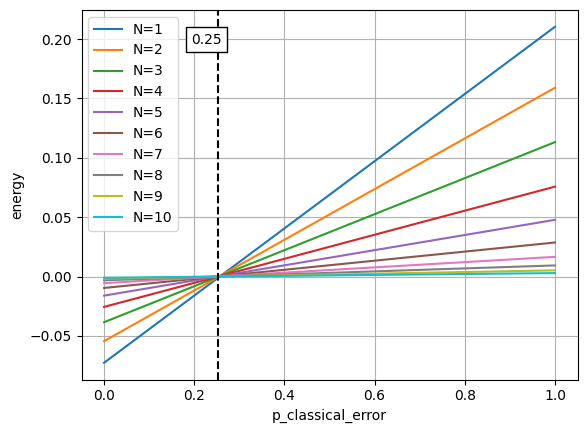
\includegraphics[width=\textwidth]{Appendix/plots/errors/numerical/Alice/Alice_energy_vs_p_class_comm_err.png}
        \caption{$H^{(1)}$}
    \end{subfigure}
    \hfill
    \begin{subfigure}[b]{0.29\textwidth}
        \centering
        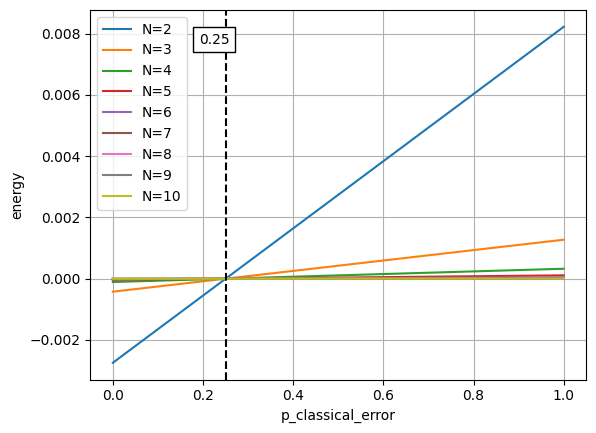
\includegraphics[width=\textwidth]{Appendix/plots/errors/numerical/NearestNeighbors/NN_X_energy_vs_p_class_comm_err.png}
        \caption{$H^{(2)}$, $\sigma_A = X_0$}
    \end{subfigure}
    \hfill
    \begin{subfigure}[b]{0.29\textwidth}
        \centering
        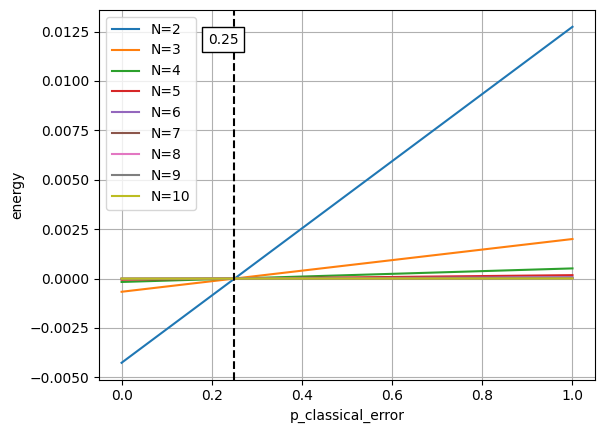
\includegraphics[width=\textwidth]{Appendix/plots/errors/numerical/NearestNeighbors/NN_Y_energy_vs_p_class_comm_err.png}
        \caption{$H^{(2)}$, $\sigma_A = Y_0$}
    \end{subfigure}

    \caption{Energy vs. Classical communication error for different \(N\) values. The linear degradation of the signal is evident across all models, with a consistent failure threshold where the expectation value crosses zero. The signal magnitude for the $H^{(2)}$ model visibly diminishes with increasing system size $N$.}
    \label{fig:energy_vs_classical_err_for_n}
\end{figure*}

\begin{figure*}[tb!]
    \centering
    \begin{subfigure}[b]{0.24\textwidth}
        \centering
        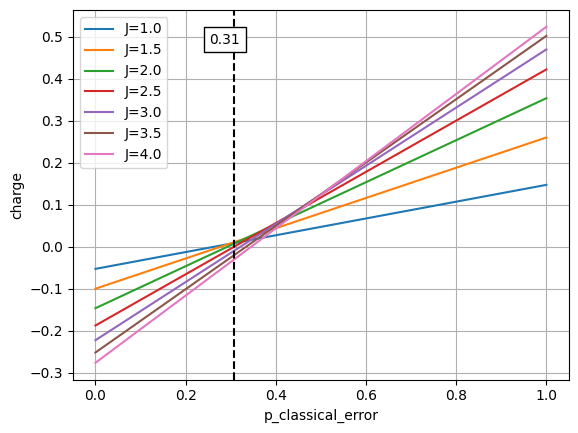
\includegraphics[width=\textwidth]{Appendix/plots/errors/numerical/Alice/N1/N1_charge_vs_p_classical_error.png}
        \caption{Charge, $N=1$}
    \end{subfigure}
    \hfill
    \begin{subfigure}[b]{0.24\textwidth}
        \centering
        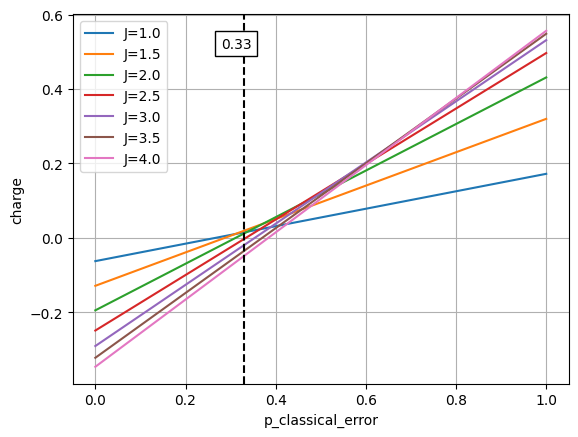
\includegraphics[width=\textwidth]{Appendix/plots/errors/numerical/Alice/N2/N2_charge_vs_p_classical_error.png}
        \caption{Charge, $N=2$}
    \end{subfigure}
    \hfill
    \begin{subfigure}[b]{0.24\textwidth}
        \centering
        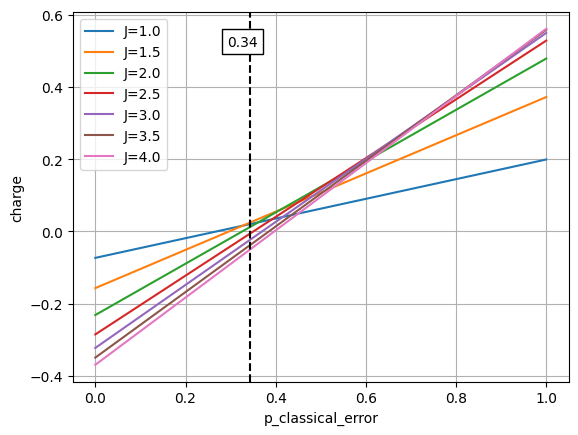
\includegraphics[width=\textwidth]{Appendix/plots/errors/numerical/Alice/N3/N3_charge_vs_p_classical_error.png}
        \caption{Charge, $N=3$}
    \end{subfigure}
    \hfill
    \begin{subfigure}[b]{0.24\textwidth}
        \centering
        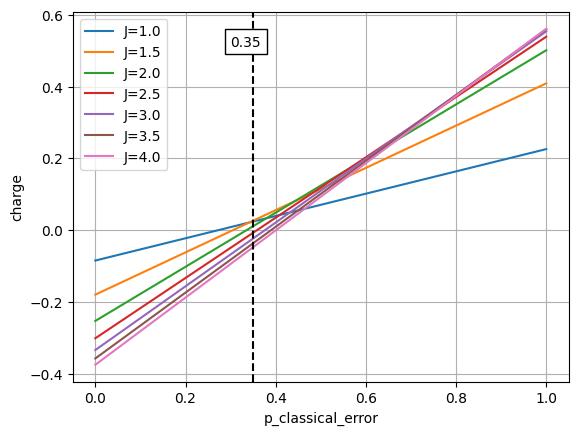
\includegraphics[width=\textwidth]{Appendix/plots/errors/numerical/Alice/N4/N4_charge_vs_p_classical_error.png}
        \caption{Charge, $N=4$}
    \end{subfigure}

    \vspace{0.5em}
    
    \begin{subfigure}[b]{0.24\textwidth}
        \centering
        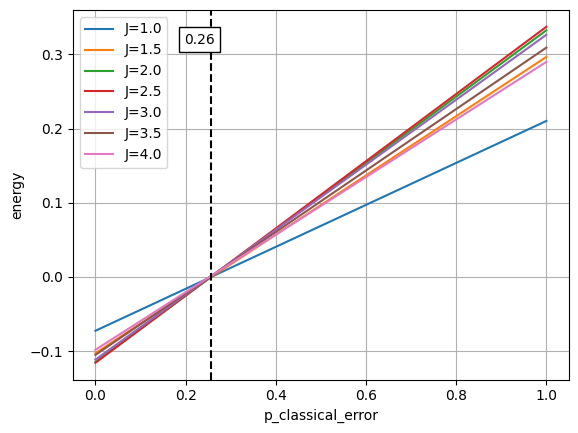
\includegraphics[width=\textwidth]{Appendix/plots/errors/numerical/Alice/N1/N1_energy_vs_p_classical_error.png}
        \caption{Energy, $N=1$}
    \end{subfigure}
    \hfill
    \begin{subfigure}[b]{0.24\textwidth}
        \centering
        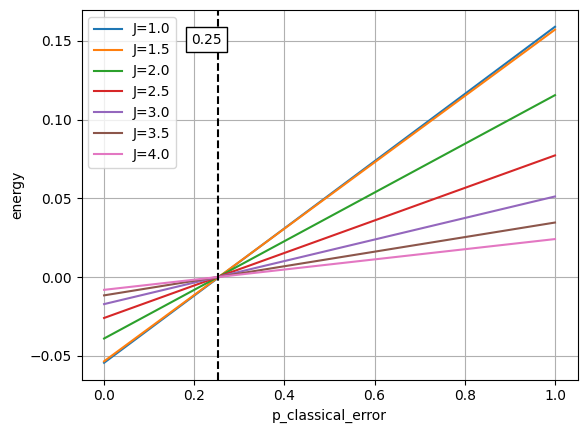
\includegraphics[width=\textwidth]{Appendix/plots/errors/numerical/Alice/N2/N2_energy_vs_p_classical_error.png}
        \caption{Energy, $N=2$}
    \end{subfigure}
    \hfill
    \begin{subfigure}[b]{0.24\textwidth}
        \centering
        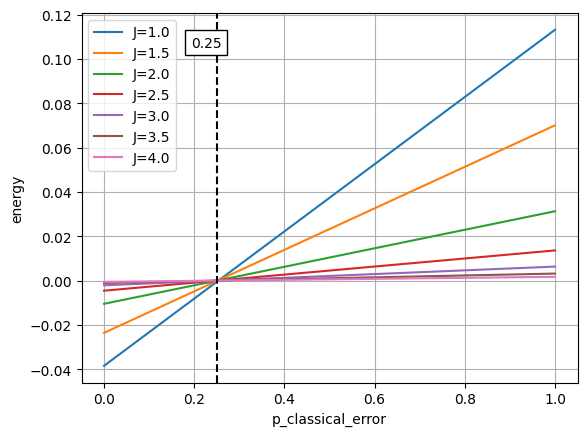
\includegraphics[width=\textwidth]{Appendix/plots/errors/numerical/Alice/N3/N3_energy_vs_p_classical_error.png}
        \caption{Energy, $N=3$}
    \end{subfigure}
    \hfill
    \begin{subfigure}[b]{0.24\textwidth}
        \centering
        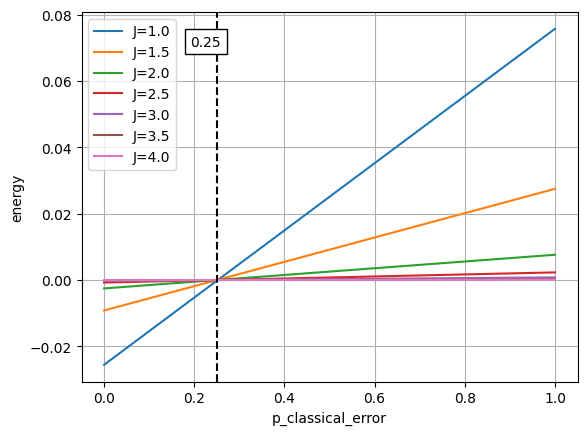
\includegraphics[width=\textwidth]{Appendix/plots/errors/numerical/Alice/N4/N4_energy_vs_p_classical_error.png}
        \caption{Energy, $N=4$}
    \end{subfigure}

    \caption{Classical communication error vs the coupling \(J\) for the star-interaction Hamiltonian $H^{(1)}$.}
    \label{fig:classical_err_alice_ham}
\end{figure*}

\begin{figure*}[tb!]
    \centering
    \begin{subfigure}[b]{0.29\textwidth}
        \centering
        
\includegraphics[width=\textwidth]{plots/errors/numerical/N2_charge_vs_p_classical_error.png}
        \caption{Charge, $N=2$}
    \end{subfigure}
    \hfill
    \begin{subfigure}[b]{0.29\textwidth}
        \centering
        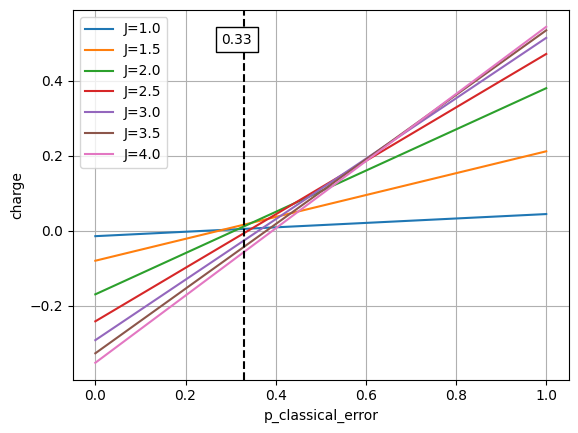
\includegraphics[width=\textwidth]{Appendix/plots/errors/numerical/NearestNeighbors/N3/X_N3_charge_vs_p_classical_error.png}
        \caption{Charge, $N=3$}
    \end{subfigure}
    \hfill
    \begin{subfigure}[b]{0.29\textwidth}
        \centering
        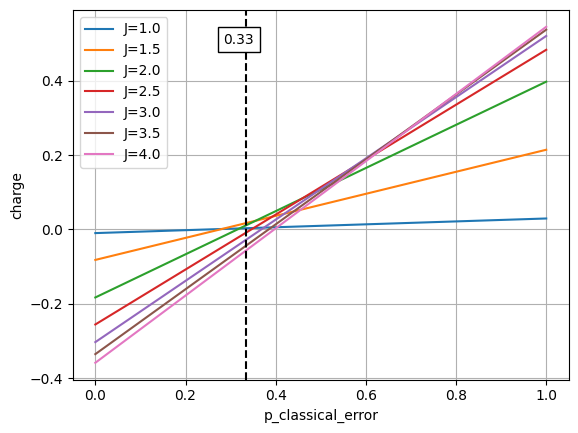
\includegraphics[width=\textwidth]{Appendix/plots/errors/numerical/NearestNeighbors/N4/X_N4_charge_vs_p_classical_error.png}
        \caption{Charge, $N=4$}
    \end{subfigure}

    \vspace{0.5em}
    
    \begin{subfigure}[b]{0.29\textwidth}
        \centering
        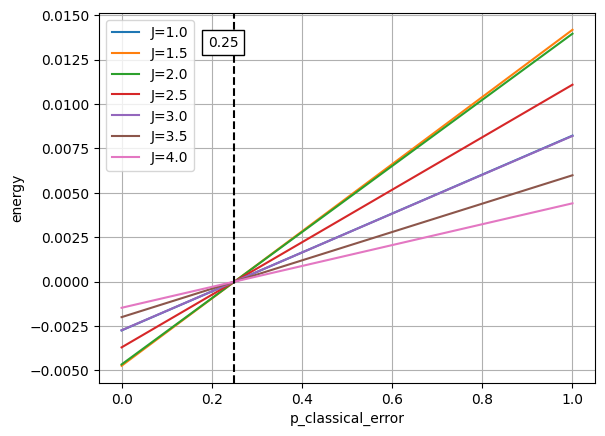
\includegraphics[width=\textwidth]{Appendix/plots/errors/numerical/NearestNeighbors/N2/X_N2_energy_vs_p_classical_error.png}
        \caption{Energy, $N=2$}
    \end{subfigure}
    \hfill
    \begin{subfigure}[b]{0.29\textwidth}
        \centering
        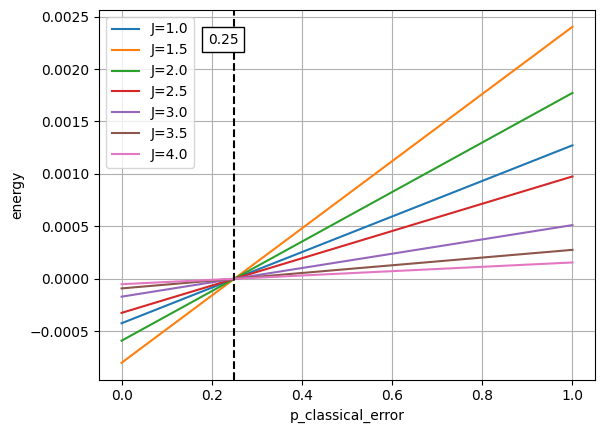
\includegraphics[width=\textwidth]{Appendix/plots/errors/numerical/NearestNeighbors/N3/X_N3_energy_vs_p_classical_error.png}
        \caption{Energy, $N=3$}
    \end{subfigure}
    \hfill
    \begin{subfigure}[b]{0.29\textwidth}
        \centering
        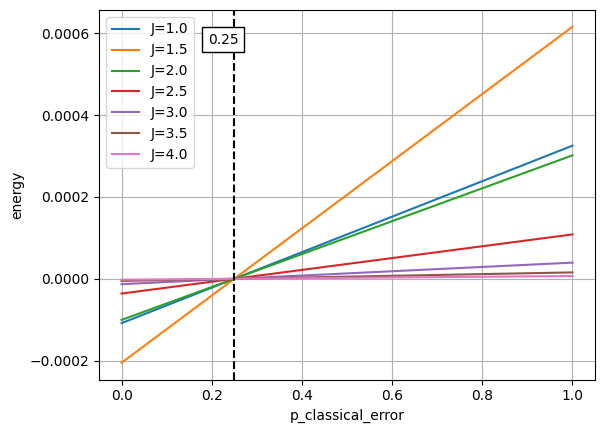
\includegraphics[width=\textwidth]{Appendix/plots/errors/numerical/NearestNeighbors/N4/X_N4_energy_vs_p_classical_error.png}
        \caption{Energy, $N=4$}
    \end{subfigure}

    \caption{Classical communication error vs the coupling \(J\) for the nearest-neighbor Hamiltonian $H^{(2)}$ with Alice Base \(\sigma_A = X_0\).}
    \label{fig:classical_err_nn_ham_x}
\end{figure*}

\begin{figure*}[tb!]
    \centering
    \begin{subfigure}[b]{0.29\textwidth}
        \centering
        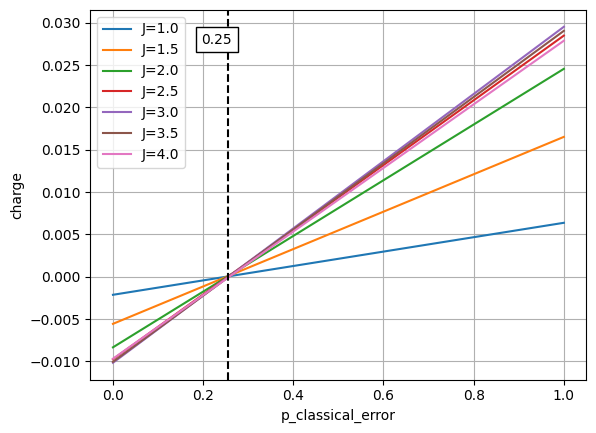
\includegraphics[width=\textwidth]{Appendix/plots/errors/numerical/NearestNeighbors/N2/Y_N2_charge_vs_p_classical_error.png}
        \caption{Charge, $N=2$}
    \end{subfigure}
    \hfill
    \begin{subfigure}[b]{0.29\textwidth}
        \centering
        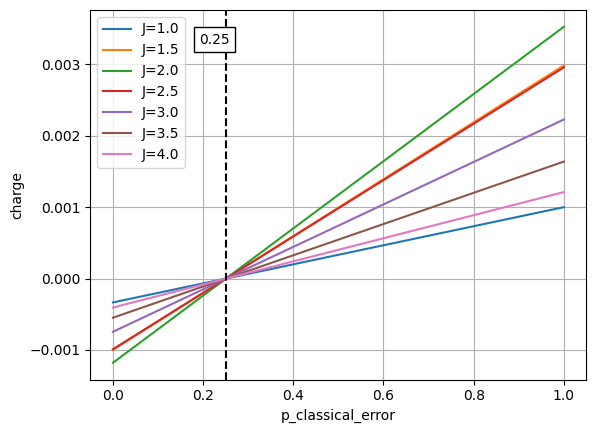
\includegraphics[width=\textwidth]{Appendix/plots/errors/numerical/NearestNeighbors/N3/Y_N3_charge_vs_p_classical_error.png}
        \caption{Charge, $N=3$}
    \end{subfigure}
    \hfill
    \begin{subfigure}[b]{0.29\textwidth}
        \centering
        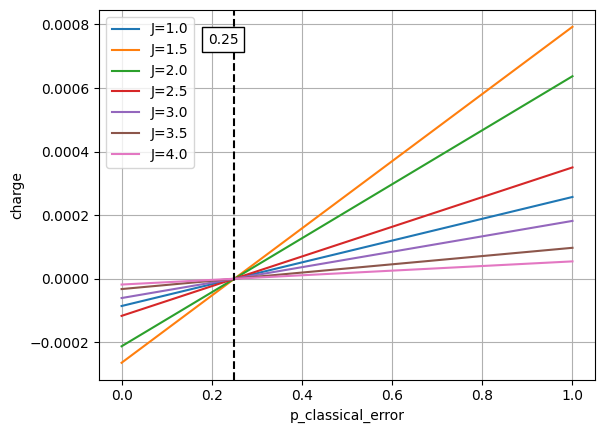
\includegraphics[width=\textwidth]{Appendix/plots/errors/numerical/NearestNeighbors/N4/Y_N4_charge_vs_p_classical_error.png}
        \caption{Charge, $N=4$}
    \end{subfigure}

    \vspace{0.5em}
    
    \begin{subfigure}[b]{0.29\textwidth}
        \centering
        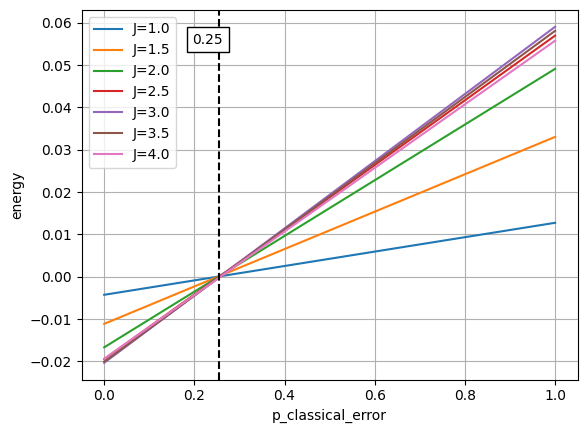
\includegraphics[width=\textwidth]{Appendix/plots/errors/numerical/NearestNeighbors/N2/Y_N2_energy_vs_p_classical_error.png}
        \caption{Energy, $N=2$}
    \end{subfigure}
    \hfill
    \begin{subfigure}[b]{0.29\textwidth}
        \centering
        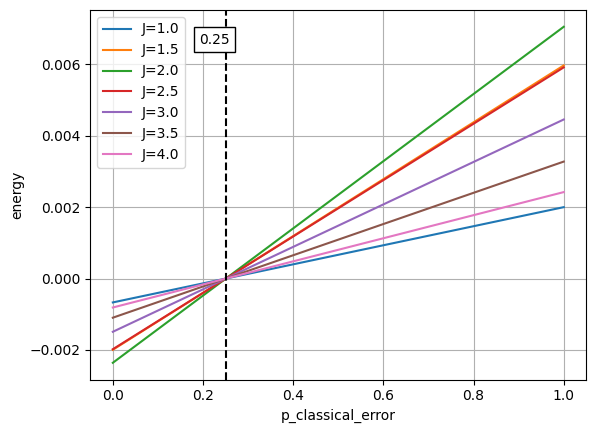
\includegraphics[width=\textwidth]{Appendix/plots/errors/numerical/NearestNeighbors/N3/Y_N3_energy_vs_p_classical_error.png}
        \caption{Energy, $N=3$}
    \end{subfigure}
    \hfill
    \begin{subfigure}[b]{0.29\textwidth}
        \centering
        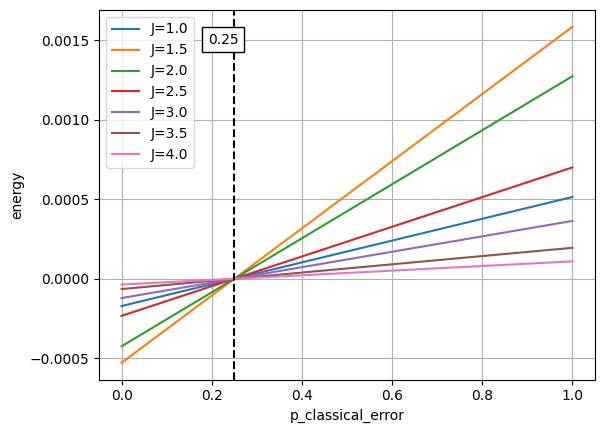
\includegraphics[width=\textwidth]{Appendix/plots/errors/numerical/NearestNeighbors/N4/Y_N4_energy_vs_p_classical_error.png}
        \caption{Energy, $N=4$}
    \end{subfigure}

    \caption{Classical communication error vs the coupling \(J\) for the nearest-neighbor Hamiltonian $H^{(2)}$ with Alice Base \(\sigma_A = Y_0\).}
    \label{fig:classical_err_nn_ham_y}
\end{figure*}

An error in the classical communication channel represents a scenario where the measurement outcome bit sent by Alice is flipped with a probability $p$ before it reaches Bob. This type of error directly impacts Bob's conditional operation, causing him to apply the incorrect unitary rotation. Consequently, the final state at Bob's side becomes a statistical mixture of the state corresponding to the intended outcome (transmitted with probability $1-p$) and the state corresponding to the flipped outcome (transmitted with probability $p$) \cite{QKDbyQET}. The resulting density matrix at Bob's site is given by:

\begin{equation*}
\begin{aligned}
\rho_{B,p} &= (1-p)\sum_{b}U_{B}(b)P_{A}(b)\rho_{gs}P_{A}(b)U_{B}^{\dagger}(b) \\
&+ p\sum_{b'=b\oplus1}U_{B}(b')P_{A}(b)\rho_{gs}P_{A}(b)U_{B}^{\dagger}(b')
\end{aligned}
\end{equation*}

This leads to a linear degradation of the expected signal, which can be expressed as \cite{QKDbyQET}:

\begin{equation*}
\langle\Delta O_{B}\rangle_{p} = (1-p)\langle\Delta O_{B}\rangle_{a=0} + p\langle\Delta O_{B}\rangle_{a=1}
\end{equation*}


Since the protocol is designed such that the intended signal $\langle\Delta O_{B}\rangle_{a=0}$ is negative and the flipped signal $\langle\Delta O_{B}\rangle_{a=1}$ is positive and of similar magnitude, the overall expectation value is attenuated linearly as $p$ increases, moving from a negative value towards a positive one. The protocol fails when this value crosses zero, as this constitutes a bit-error in the generated key, rendering it insecure.

The numerical results presented in Figure \ref{fig:energy_vs_classical_err_for_n} and Figures \ref{fig:classical_err_alice_ham}-\ref{fig:classical_err_nn_ham_y} comprehensively illustrate this behavior across all simulated configurations.

Figure \ref{fig:energy_vs_classical_err_for_n} shows the teleported energy as a function of the error probability $p$ for various system sizes $N$. For all Hamiltonians, the expected linear decay is observed. A critical failure threshold, where the sign of the teleported energy flips, consistently appears around $p \approx 0.25$, corroborating the analysis in \cite{QKDbyQET}. Notably, for the nearest-neighbor model ($H^{(2)}$), the magnitude of the teleported energy signal weakens significantly as the system size $N$ increases, which makes resolving the signal from noise more challenging in larger systems.

Figures \ref{fig:classical_err_alice_ham}, \ref{fig:classical_err_nn_ham_x}, and \ref{fig:classical_err_nn_ham_y} provide a more detailed view, showing the behavior for different coupling strengths $J$.
\begin{itemize}
    \item \textbf{Star-Interaction Model ($H^{(1)}$):} As shown in Figure \ref{fig:classical_err_alice_ham}, both energy and charge signals exhibit a clear linear decay. The slope of this decay is dependent on the coupling strength $J$, with stronger couplings (which produce a larger initial signal magnitude at $p=0$) leading to a steeper decline. Despite this, the sign-flip threshold is remarkably stable across different couplings and system sizes, occurring around $p \approx 0.28$ for charge and $p \approx 0.25$ for energy. This is consistent with the findings in \cite{QKDbyQET}.

    \item \textbf{Nearest-Neighbor Model ($H^{(2)}$):} The results for this model, depicted in Figures \ref{fig:classical_err_nn_ham_x} ($\sigma_A = X_0$) and \ref{fig:classical_err_nn_ham_y} ($\sigma_A = Y_0$), confirm a similar linear degradation. However, a key distinction emerges: the charge signal's magnitude remains more robust against increases in system size $N$ compared to the energy signal. While the fundamental error threshold remains in the same $p \approx 0.25-0.32$ range, the rapid decay of the energy signal's absolute value means that for larger distances between Alice and Bob, the charge-based protocol provides a more resilient and discernible signal. This highlights a significant practical advantage of charge teleportation for implementing QKD in larger, more realistic quantum systems.
\end{itemize}

In summary, while the protocol is fundamentally vulnerable to classical communication errors with a consistent failure threshold, the charge teleportation protocol demonstrates superior stability and resilience, especially in the nearest-neighbor model, where its signal magnitude degrades less rapidly with system size compared to energy teleportation. This makes it a more robust choice for practical implementations.

\subsection{Mixture with an Excited State}

\input{Appendix/noise-errors/excited-mixture}

Perfect ground state preparation is experimentally challenging; a common imperfection is a residual population of excited states. This section analyzes the protocol's performance when the initial resource state is not the pure ground state $\rho_{gs} = |gs\rangle\langle gs|$, but rather a statistical mixture with the first excited state, $\rho_1$. This error model is particularly relevant for systems with a small energy gap, where distinguishing the ground state from low-lying excitations is difficult \cite{QKDbyQET}. The state is modeled as:
\begin{equation*}
\rho = (1-p)\rho_{gs} + p\rho_1
\end{equation*}
where $p$ is the probability of the system being in the excited state. The teleported signal becomes a weighted average of the contributions from each state, and the change in Bob's local energy is given by \cite{QKDbyQET}:
\begin{equation*}
\langle\Delta H_B\rangle_p = (1-p)\text{Tr}[(\rho_B - \rho_{gs})H_B] + p\,\text{Tr}[(\sigma_B - \sigma)H_B]
\end{equation*}
where $\rho_B$ and $\sigma_B$ are the final states at Bob's side originating from the ground and excited states, respectively.

Our analysis, presented in Figures \ref{fig:alice_num_mixture_error_appendix} through \ref{fig:nn_qiskit_mixture_error_appendix}, reveals a critical performance difference between the energy and charge teleportation protocols under this noise model.

A crucial insight is that energy teleportation is highly vulnerable to this error. Low-lying excitations significantly alter the local energy expectation value $\langle H_B \rangle$, often contributing a large positive offset that overwhelms the negative teleported signal from the ground state component \cite{QKDbyQET}. This causes the total signal to rapidly cross zero and become positive, even for moderate error probabilities ($p \approx 0.15-0.29$), as seen in the top rows of Figures \ref{fig:alice_num_mixture_error_appendix}, \ref{fig:nn_X_num_mixture_error_appendix}, and \ref{fig:nn_Y_num_mixture_error_appendix}. Such a sign-flip is fatal to the QKD protocol.

In contrast, the charge protocol is far more robust. The charge observable $Q_B$, being related to local spin parity rather than total energy, is less sensitive to such energy shifts. The quantum correlations responsible for charge teleportation often retain their sign and structure across low-energy states. As a result, the contribution from the excited state does not introduce a large positive offset. The charge signal therefore remains negative across a wide range of mixture probabilities, merely decreasing in magnitude as $p$ increases. This remarkable stability is evident in the bottom rows of all numerical simulation figures, demonstrating a decisive advantage for practical QKD.

The Qiskit simulations, shown in Figures \ref{fig:alice_qiskit_mixture_error_appendix} and \ref{fig:nn_qiskit_mixture_error_appendix}, corroborate these numerical findings. They also highlight the practical measurement challenges: the energy plots exhibit significant statistical variance, which is a direct consequence of both the weaker signal and the error propagation from measuring non-commuting terms in separate circuits (see Appendix F). The charge plots, in comparison, are markedly smoother, underscoring not only its theoretical robustness against this error model but also its superior statistical stability in a measurement context. This trend holds across all tested Hamiltonians and system sizes.

\subsection{Superposition with an Excited State}

\begin{figure*}[tb!]
    \centering
    \subfloat[Energy, \( N = 2 \)]{
        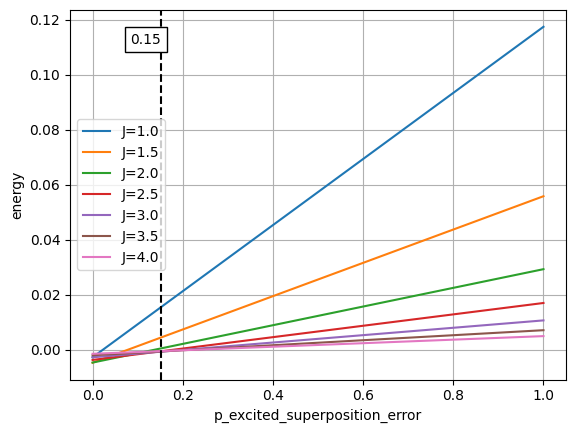
\includegraphics[width=0.3\textwidth]{Appendix/plots/errors/numerical/NearestNeighbors/N2/X_N2_energy_vs_p_excited_superposition_error.png}
    }
    \hfill
    \subfloat[Energy, \( N = 3 \)]{
        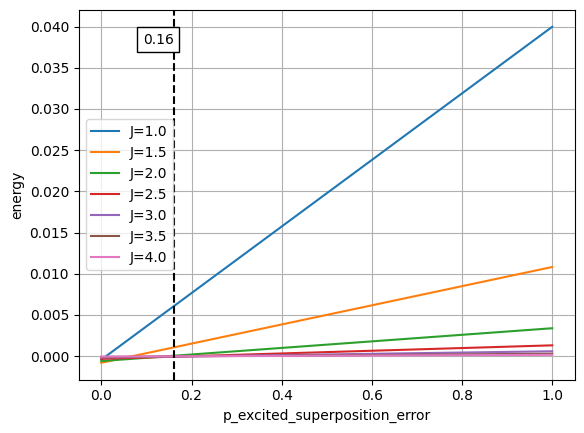
\includegraphics[width=0.3\textwidth]{Appendix/plots/errors/numerical/NearestNeighbors/N3/X_N3_energy_vs_p_excited_superposition_error.png}
    }
    \hfill
    \subfloat[Energy, \( N = 4 \)]{
        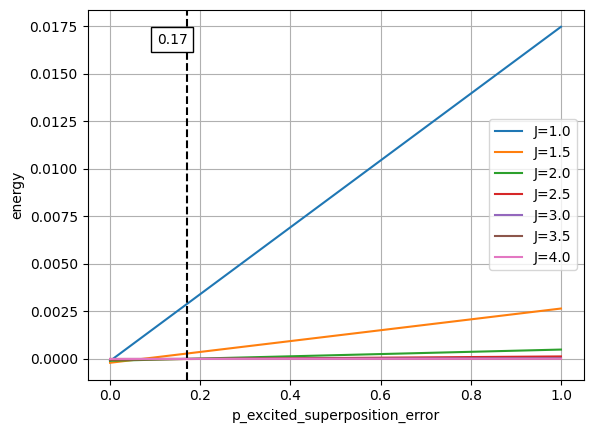
\includegraphics[width=0.3\textwidth]{Appendix/plots/errors/numerical/NearestNeighbors/N4/X_N4_energy_vs_p_excited_superposition_error.png}
    }

    \vspace{0.5em}

    \subfloat[Charge, \( N = 2 \)]{
        
\includegraphics[width=0.3\textwidth]{plots/errors/numerical/N2_charge_vs_p_excited_superposition_error.png}
    }
    \hfill
    \subfloat[Charge, \( N = 3 \)]{
        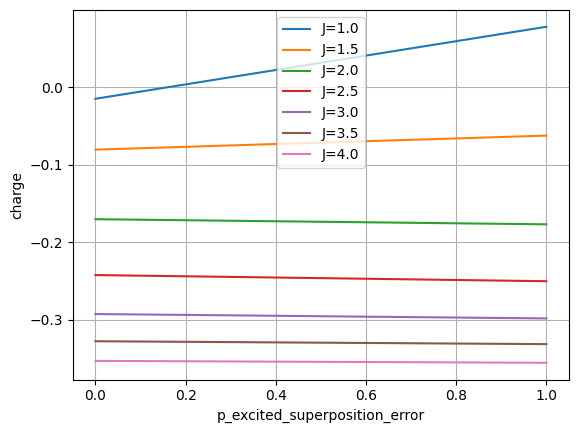
\includegraphics[width=0.3\textwidth]{Appendix/plots/errors/numerical/NearestNeighbors/N3/X_N3_charge_vs_p_excited_superposition_error.png}
    }
    \hfill
    \subfloat[Charge, \( N = 4 \)]{
        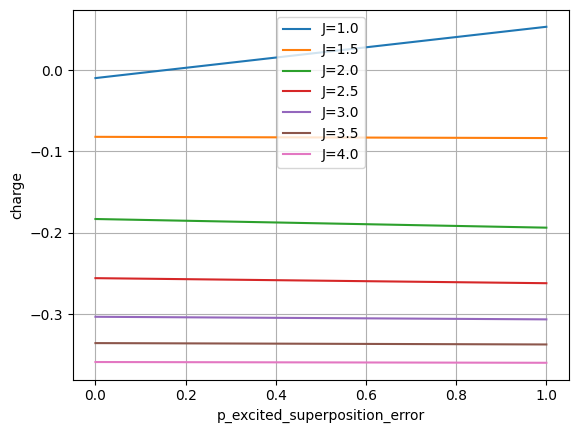
\includegraphics[width=0.3\textwidth]{Appendix/plots/errors/numerical/NearestNeighbors/N4/X_N4_charge_vs_p_excited_superposition_error.png}
    }
    
    \caption{Numerical simulation results for teleported expectation value vs. the probability $p$ of superposition with the first excited state for Nearest Neighbors Hamiltonian \(H^{(2)}\) with Alice base \(\sigma_A = X_0\).}
    \label{fig:nn_X_num_superposition_error_appendix}
\end{figure*}

\begin{figure*}[tb!]
    \centering
    \subfloat[Energy, \( N = 2 \)]{
        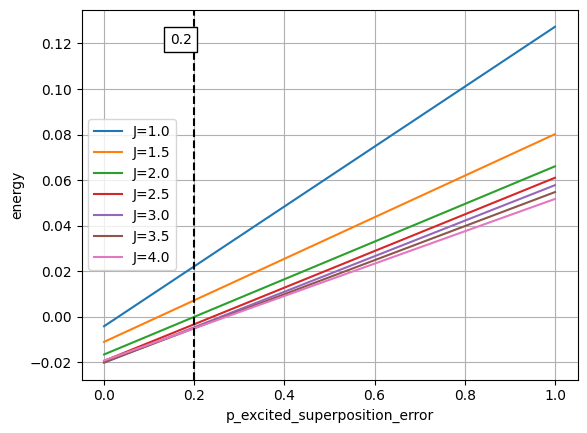
\includegraphics[width=0.3\textwidth]{Appendix/plots/errors/numerical/NearestNeighbors/N2/Y_N2_energy_vs_p_excited_superposition_error.png}
    }
    \hfill
    \subfloat[Energy, \( N = 3 \)]{
        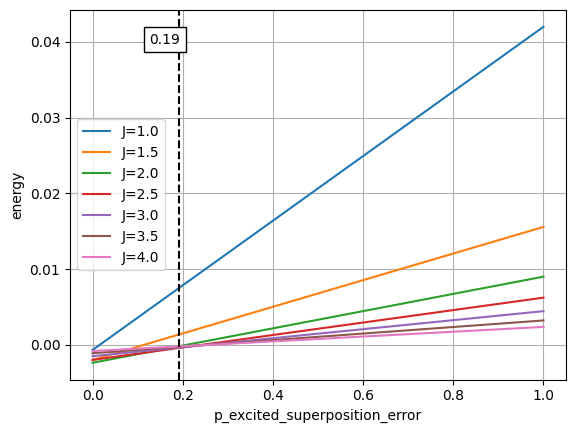
\includegraphics[width=0.3\textwidth]{Appendix/plots/errors/numerical/NearestNeighbors/N3/Y_N3_energy_vs_p_excited_superposition_error.png}
    }
    \hfill
    \subfloat[Energy, \( N = 4 \)]{
        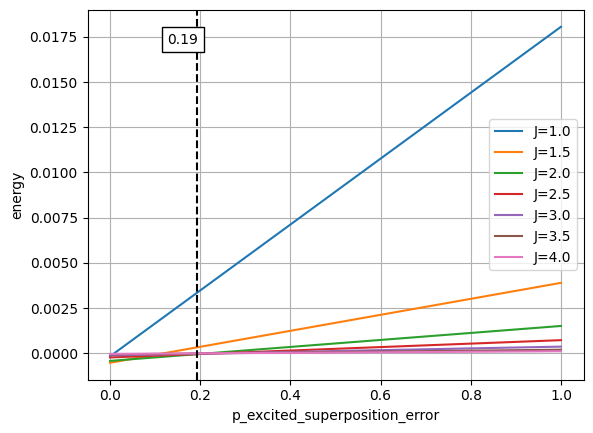
\includegraphics[width=0.3\textwidth]{Appendix/plots/errors/numerical/NearestNeighbors/N4/Y_N4_energy_vs_p_excited_superposition_error.png}
    }

    \vspace{0.5em}

    \subfloat[Charge, \( N = 2 \)]{
        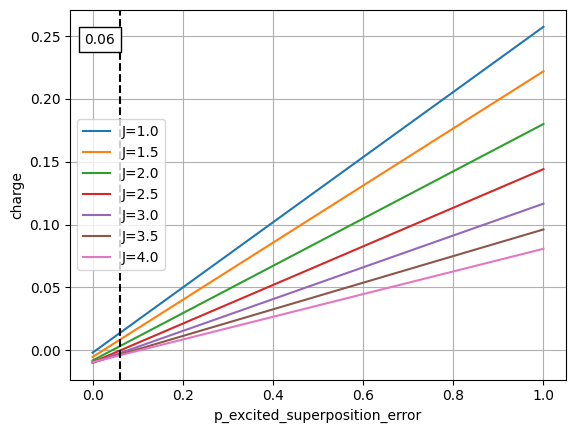
\includegraphics[width=0.3\textwidth]{Appendix/plots/errors/numerical/NearestNeighbors/N2/Y_N2_charge_vs_p_excited_superposition_error.png}
    }
    \hfill
    \subfloat[Charge, \( N = 3 \)]{
        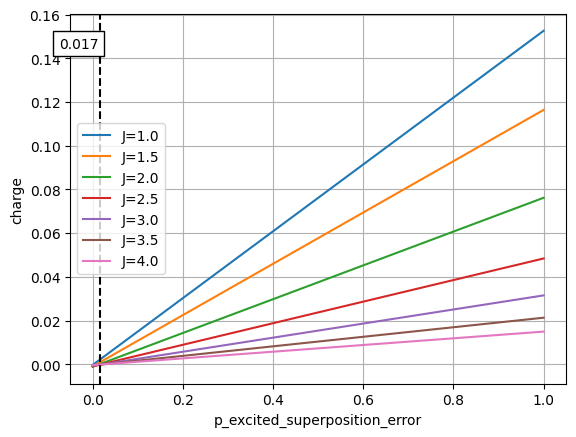
\includegraphics[width=0.3\textwidth]{Appendix/plots/errors/numerical/NearestNeighbors/N3/Y_N3_charge_vs_p_excited_superposition_error.png}
    }
    \hfill
    \subfloat[Charge, \( N = 4 \)]{
        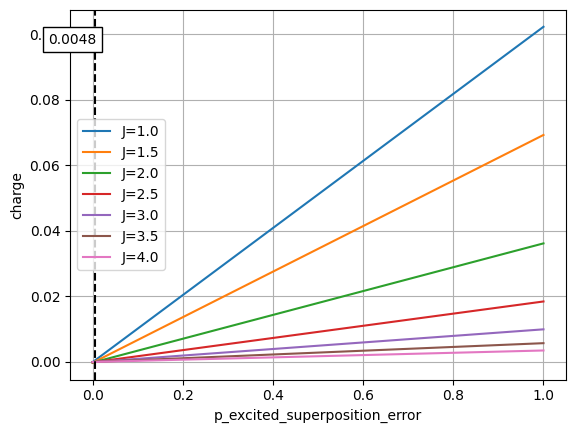
\includegraphics[width=0.3\textwidth]{Appendix/plots/errors/numerical/NearestNeighbors/N4/Y_N4_charge_vs_p_excited_superposition_error.png}
    }
    
    \caption{Numerical simulation results for teleported expectation value vs. the probability $p$ of superposition with the first excited state for Nearest Neighbors Hamiltonian \(H^{(2)}\) with Alice base \(\sigma_A = Y_0\).}
    \label{fig:nn_Y_num_superposition_error_appendix}
\end{figure*}

\begin{figure*}[tb!]
    \centering
    \subfloat[Energy, \( N = 2 \), \( \sigma_A = X_0 \)]{
        
\includegraphics[width=0.225\textwidth]{Appendix/plots/errors/qiskit/NearestNeighbors/N2/X_N2_energy_vs_p_excited_superposition_error.png}
    }
    \hfill
    \subfloat[Energy, \( N = 3 \), \( \sigma_A = X_0 \)]{
        
\includegraphics[width=0.225\textwidth]{Appendix/plots/errors/qiskit/NearestNeighbors/N3/X_N3_energy_vs_p_excited_superposition_error.png}
    }
    \hfill
    \subfloat[Charge, \( N = 2 \), \( \sigma_A = X_0 \)]{
        
\includegraphics[width=0.225\textwidth]{plots/errors/qiskit/N2_charge_vs_p_excited_superposition_error.png}
    }
    \hfill
    \subfloat[Charge, \( N = 3 \), \( \sigma_A = X_0 \)]{
        
\includegraphics[width=0.225\textwidth]{Appendix/plots/errors/qiskit/NearestNeighbors/N3/X_N3_charge_vs_p_excited_superposition_error.png}
    }

    \vspace{0.5em}

    \subfloat[Energy, \( N = 2 \), \( \sigma_A = Y_0 \)]{
        
\includegraphics[width=0.225\textwidth]{Appendix/plots/errors/qiskit/NearestNeighbors/N2/Y_N2_energy_vs_p_excited_superposition_error.png}
    }
    \hfill
    \subfloat[Energy, \( N = 3 \), \( \sigma_A = Y_0 \)]{
        
\includegraphics[width=0.225\textwidth]{Appendix/plots/errors/qiskit/NearestNeighbors/N3/Y_N3_energy_vs_p_excited_superposition_error.png}
    }
    \hfill
    \subfloat[Charge, \( N = 2 \), \( \sigma_A = Y_0 \)]{
        
\includegraphics[width=0.225\textwidth]{Appendix/plots/errors/qiskit/NearestNeighbors/N2/Y_N2_charge_vs_p_excited_superposition_error.png}
    }
    \hfill
    \subfloat[Charge, \( N = 3 \), \( \sigma_A = Y_0 \)]{
        
\includegraphics[width=0.225\textwidth]{Appendix/plots/errors/qiskit/NearestNeighbors/N3/Y_N3_charge_vs_p_excited_superposition_error.png}
    }
    
    \caption{Qiskit simulation results for teleported expectation value vs. the probability $p$ of superposition with the first excited state for Nearest Neighbors Hamiltonian \(H^{(2)}\) for both Alice bases.}
    \label{fig:nn_qiskit_superposition_error_appendix}
\end{figure*}


A coherent error in state preparation can result in a superposition of the ground state $\ket{\psi_{gs}}$ and the first excited state $\ket{\psi_{1}}$. Unlike a statistical mixture, this creates a pure state with contributions from both energy levels, modeled as:
\begin{equation*}
\ket{\psi} = \sqrt{1-p}\ket{\psi_{gs}} + e^{i\alpha}\sqrt{p}\ket{\psi_{1}}
\end{equation*}
where $p$ is the probability of the excited state amplitude and $\alpha$ is a relative phase. As shown in \cite{QKDbyQET}, the effect of the phase $\alpha$ is generally negligible, so the analysis focuses on the impact of the probability $p$.

The key distinction of this coherent error is the introduction of interference terms (e.g., cross-terms involving $\bra{\psi_{gs}}...\ket{\psi_{1}}$) into the expectation values of the parameters $\xi$ and $\eta$ that govern the teleportation protocol. This leads to a non-linear degradation of the signal as a function of $p$, which is a distinct signature of a coherent error. The phase sensitivity inherent in the superposition can cause destructive interference that is particularly detrimental to the commutator term $\eta$, which is the primary driver of the teleportation process.

The trend, shown across Figures \ref{fig:alice_num_superposition_error_appendix} to \ref{fig:nn_qiskit_superposition_error_appendix}, is qualitatively similar to the statistical mixture case but quantitatively distinct due to the non-linear signal degradation. Once again, the energy protocol proves highly susceptible to this error, with the signal quickly flipping to positive at low error probabilities. The charge protocol, however, demonstrates significant resilience. The correlations enabling charge teleportation are less affected by this coherent mixing, allowing the signal to maintain its negative sign and thus preserve the integrity of the key bit across a much wider range of $p$.

The Qiskit simulations presented in Figures \ref{fig:alice_qiskit_superposition_error_appendix} and \ref{fig:nn_qiskit_superposition_error_appendix} confirm these non-linear trends. The increased statistical variance in the plots, particularly for the energy observable in the nearest-neighbor model, makes it challenging to precisely resolve the non-linear signal from finite-shot noise. This observation reinforces that the charge protocol is not only more robust to the underlying physical error but also more statistically stable in a realistic measurement scenario.

\subsection{Bit-Flip Error}

\input{Appendix/noise-errors/bitfilp}

We now consider the effect of a local bit-flip error channel on the shared resource state. This error is modeled by the transformation $\rho \rightarrow (1-p)\rho + pX_{n}\rho X_{n}$, which applies a Pauli-\(X\) gate to the qubit at site $n$ with probability $p$. Due to the local nature of the protocol's key operators, it is sufficient to analyze the impact of such errors occurring at Alice's site ($n=0$) and Bob's site ($n=N$) \cite{QKDbyQET}.

A remarkable feature of the protocol is its inherent robustness to bit-flip errors on Alice's qubit when she measures in the corresponding basis. If a bit-flip error ($X_0$) occurs on Alice's qubit in the resource state before her measurement in the $\sigma_A = X_0$ basis, it has no effect on Bob's final expectation value. This is because the measurement operator $P_A(b)$ projects the state onto an eigenstate of $X_0$. Since the error operator $X_0$ commutes with the measurement projectors, the term corresponding to the error state, $P_A(b)X_0\rho_{gs}X_0P_A(b)$, reduces to $P_A(b)\rho_{gs}P_A(b)$, making the error undetectable and harmless in this specific configuration.

The more impactful scenario is a bit-flip error on Bob's qubit, which directly corrupts the entangled correlations he needs to perform his operation. This error attenuates the signal by degrading the non-local correlations in the ground state. As shown in the numerical simulations in Figures \ref{fig:alice_num_bitflip_error_appendix}, \ref{fig:nn_X_num_bitflip_error_appendix}, and \ref{fig:nn_Y_num_bitflip_error_appendix}, both the energy and charge signals decay smoothly as the error probability $p$ increases. Unlike the state preparation errors, bit-flips do not introduce a large offsetting term that causes a premature sign-flip. Instead, the failure is gradual, manifesting as a reduced signal-to-noise ratio. While the energy protocol often yields a larger absolute signal, both observables exhibit a similar resilience characterized by this smooth degradation.

The Qiskit simulations presented in Figures \ref{fig:alice_qiskit_bitflip_error_appendix} and \ref{fig:nn_qiskit_bitflip_error_appendix} validate these numerical findings. The results show a stable decay, confirming that the protocol's relative robustness to bit-flip errors on Bob's qubit is well-represented at the quantum circuit level \cite{Lo2005, Wang2005}.

\subsection{Alice site Phase-Flip Error}

\WarningFilter{latex}{Text page 31 contains only floats}

\begin{figure*}[tb!]
    \centering
    \begin{subfigure}[b]{0.2\textwidth}
        \centering
        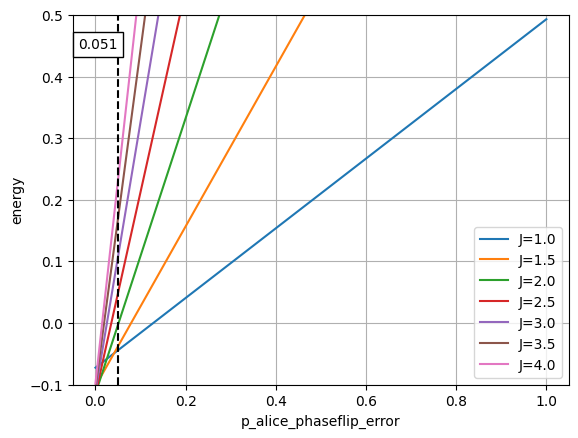
\includegraphics[width=\textwidth]{Appendix/plots/errors/numerical/Alice/N1/N1_energy_vs_p_alice_phaseflip_error.png}
        \caption{Energy, $N=1$}
    \end{subfigure}
    \hfill
    \begin{subfigure}[b]{0.2\textwidth}
        \centering
        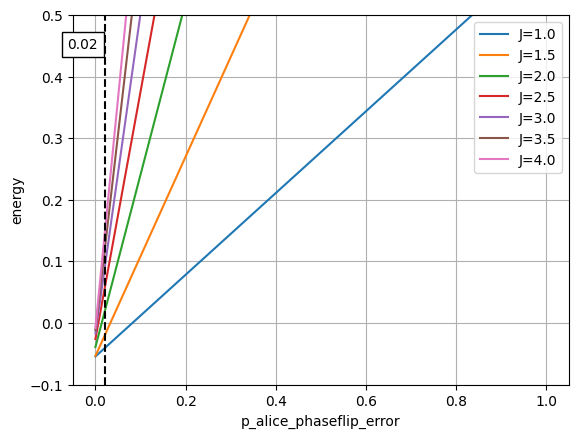
\includegraphics[width=\textwidth]{Appendix/plots/errors/numerical/Alice/N2/N2_energy_vs_p_alice_phaseflip_error.png}
        \caption{Energy, $N=2$}
    \end{subfigure}
    \hfill
    \begin{subfigure}[b]{0.2\textwidth}
        \centering
        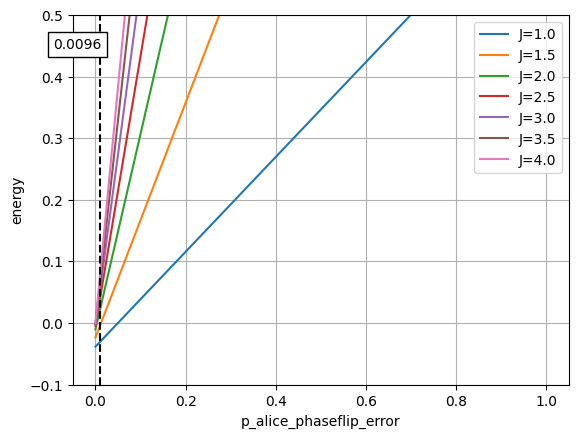
\includegraphics[width=\textwidth]{Appendix/plots/errors/numerical/Alice/N3/N3_energy_vs_p_alice_phaseflip_error.png}
        \caption{Energy, $N=3$}
    \end{subfigure}
    \hfill
    \begin{subfigure}[b]{0.2\textwidth}
        \centering
        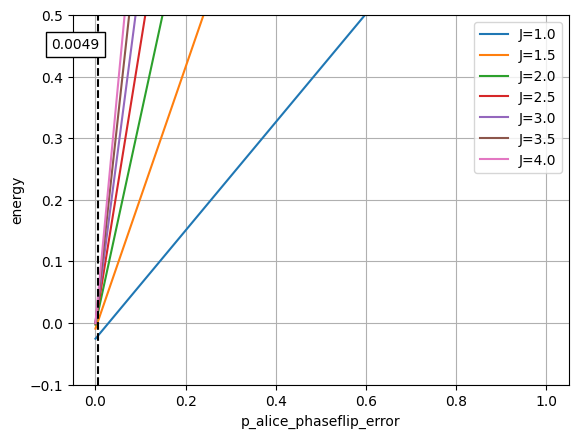
\includegraphics[width=\textwidth]{Appendix/plots/errors/numerical/Alice/N4/N4_energy_vs_p_alice_phaseflip_error.png}
        \caption{Energy, $N=4$}
    \end{subfigure}

    \vspace{0.5em}

    \begin{subfigure}[b]{0.2\textwidth}
        \centering
        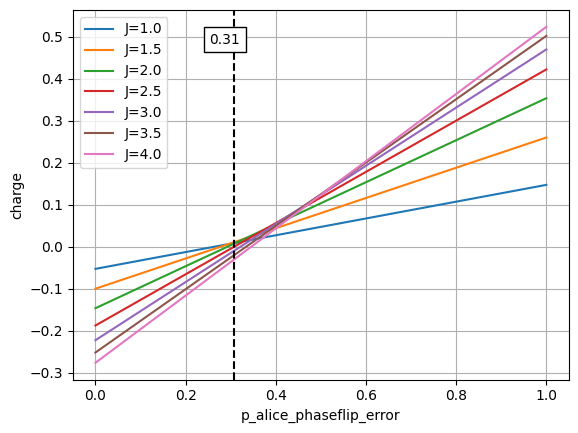
\includegraphics[width=\textwidth]{Appendix/plots/errors/numerical/Alice/N1/N1_charge_vs_p_alice_phaseflip_error.png}
        \caption{Charge, $N=1$}
    \end{subfigure}
    \hfill
    \begin{subfigure}[b]{0.2\textwidth}
        \centering
        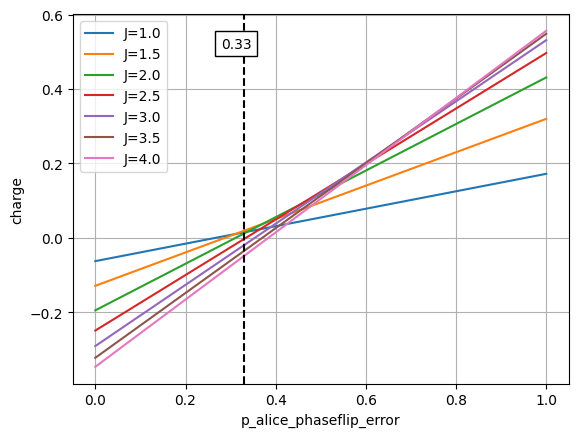
\includegraphics[width=\textwidth]{Appendix/plots/errors/numerical/Alice/N2/N2_charge_vs_p_alice_phaseflip_error.png}
        \caption{Charge, $N=2$}
    \end{subfigure}
    \hfill
    \begin{subfigure}[b]{0.2\textwidth}
        \centering
        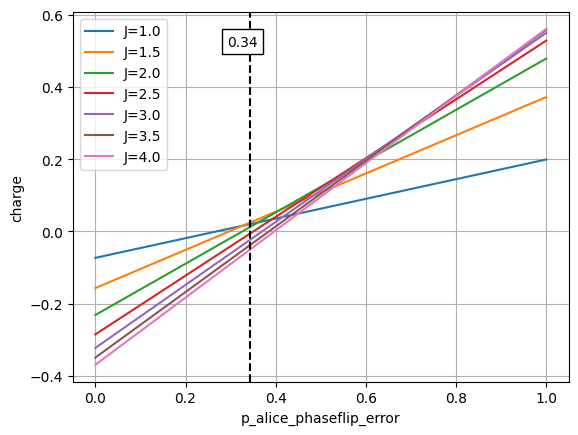
\includegraphics[width=\textwidth]{Appendix/plots/errors/numerical/Alice/N3/N3_charge_vs_p_alice_phaseflip_error.png}
        \caption{Charge, $N=3$}
    \end{subfigure}
    \hfill
    \begin{subfigure}[b]{0.2\textwidth}
        \centering
        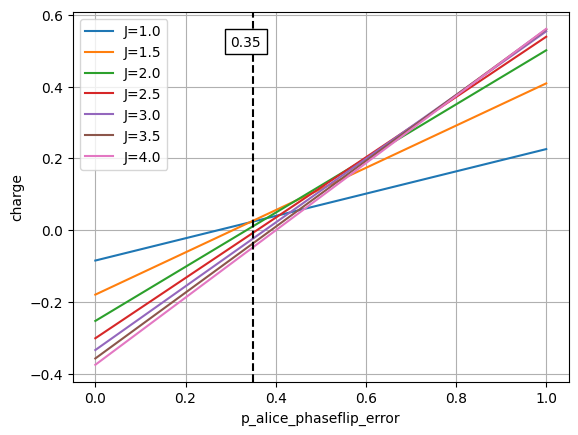
\includegraphics[width=\textwidth]{Appendix/plots/errors/numerical/Alice/N4/N4_charge_vs_p_alice_phaseflip_error.png}
        \caption{Charge, $N=4$}
    \end{subfigure}
    
    \caption{Numerical simulation results for teleported expectation value vs. the probability $p$ of phaseflip at Alice's site for Star-Interaction Hamiltonian \(H^{(1)}\).}
    \label{fig:alice_num_alice_phaseflip_error_appendix}
\end{figure*}

\begin{figure*}[tb!]
    \centering
    \begin{subfigure}[b]{0.33\textwidth}
        \centering
        
\includegraphics[width=\textwidth]{Appendix/plots/errors/qiskit/Alice/N1/N1_energy_vs_p_alice_phaseflip_error.png}
        \caption{Energy, $N=1$}
    \end{subfigure}
    \hfill
    \begin{subfigure}[b]{0.33\textwidth}
        \centering
        
\includegraphics[width=\textwidth]{Appendix/plots/errors/qiskit/Alice/N2/N2_energy_vs_p_alice_phaseflip_error.png}
        \caption{Energy, $N=2$}
    \end{subfigure}
    \hfill
    \begin{subfigure}[b]{0.33\textwidth}
        \centering
        
\includegraphics[width=\textwidth]{Appendix/plots/errors/qiskit/Alice/N3/N3_energy_vs_p_alice_phaseflip_error.png}
        \caption{Energy, $N=3$}
    \end{subfigure}

    \vspace{0.5em}

    \begin{subfigure}[b]{0.33\textwidth}
        \centering
        
\includegraphics[width=\textwidth]{Appendix/plots/errors/qiskit/Alice/N1/N1_charge_vs_p_alice_phaseflip_error.png}
        \caption{Charge, $N=1$}
    \end{subfigure}
    \hfill
    \begin{subfigure}[b]{0.33\textwidth}
        \centering
        
\includegraphics[width=\textwidth]{Appendix/plots/errors/qiskit/Alice/N2/N2_charge_vs_p_alice_phaseflip_error.png}
        \caption{Charge, $N=2$}
    \end{subfigure}
    \hfill
    \begin{subfigure}[b]{0.33\textwidth}
        \centering
        
\includegraphics[width=\textwidth]{Appendix/plots/errors/qiskit/Alice/N3/N3_charge_vs_p_alice_phaseflip_error.png}
        \caption{Charge, $N=3$}
    \end{subfigure}
    
    \caption{Qiskit simulation results for teleported expectation value vs. the probability $p$ of phaseflip at Alice's site for Star-Interaction Hamiltonian \(H^{(1)}\).}
    \label{fig:alice_qiskit_alice_phaseflip_error_appendix}
\end{figure*}

\begin{figure*}[tb!]
    \centering
    \begin{subfigure}[b]{0.29\textwidth}
        \centering
        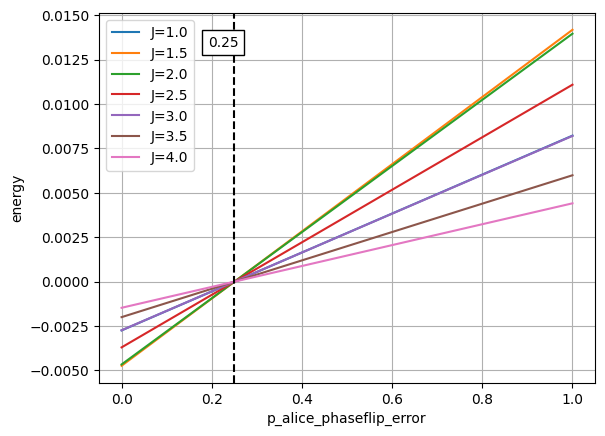
\includegraphics[width=\textwidth]{Appendix/plots/errors/numerical/NearestNeighbors/N2/X_N2_energy_vs_p_alice_phaseflip_error.png}
        \caption{Energy, $N=2$}
    \end{subfigure}
    \hfill
    \begin{subfigure}[b]{0.29\textwidth}
        \centering
        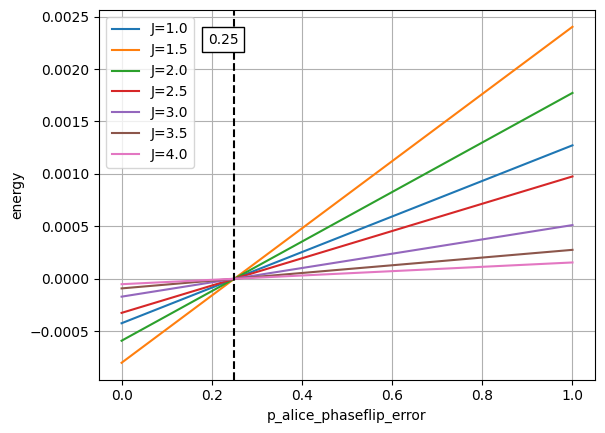
\includegraphics[width=\textwidth]{Appendix/plots/errors/numerical/NearestNeighbors/N3/X_N3_energy_vs_p_alice_phaseflip_error.png}
        \caption{Energy, $N=3$}
    \end{subfigure}
    \hfill
    \begin{subfigure}[b]{0.29\textwidth}
        \centering
        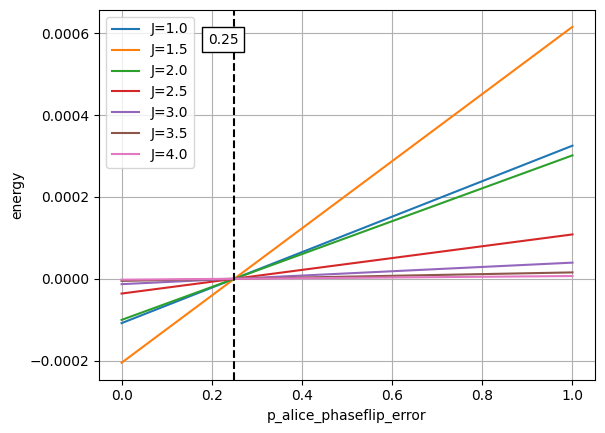
\includegraphics[width=\textwidth]{Appendix/plots/errors/numerical/NearestNeighbors/N4/X_N4_energy_vs_p_alice_phaseflip_error.png}
        \caption{Energy, $N=4$}
    \end{subfigure}

    \vspace{0.5em}

    \begin{subfigure}[b]{0.29\textwidth}
        \centering
        
\includegraphics[width=\textwidth]{plots/errors/numerical/N2_charge_vs_p_alice_phaseflip_error.png}
        \caption{Charge, $N=2$}
    \end{subfigure}
    \hfill
    \begin{subfigure}[b]{0.29\textwidth}
        \centering
        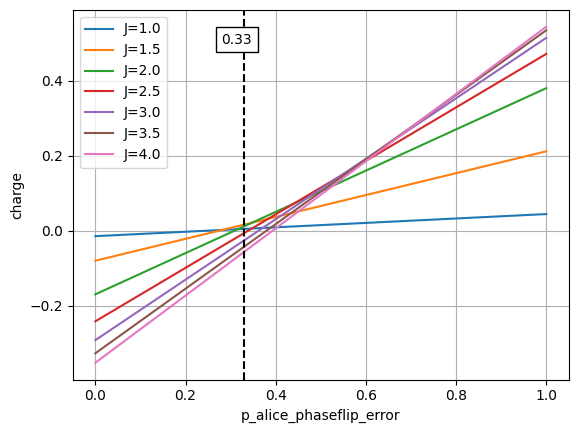
\includegraphics[width=\textwidth]{Appendix/plots/errors/numerical/NearestNeighbors/N3/X_N3_charge_vs_p_alice_phaseflip_error.png}
        \caption{Charge, $N=3$}
    \end{subfigure}
    \hfill
    \begin{subfigure}[b]{0.29\textwidth}
        \centering
        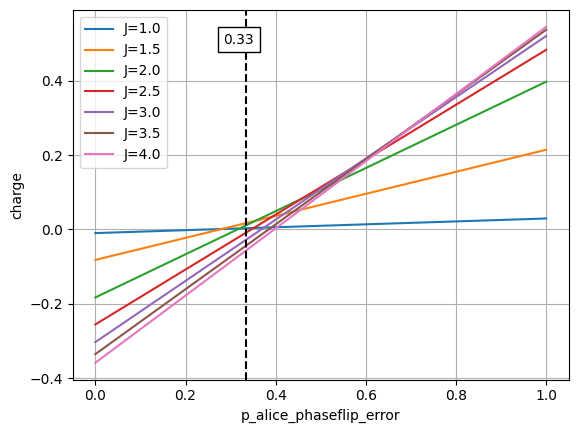
\includegraphics[width=\textwidth]{Appendix/plots/errors/numerical/NearestNeighbors/N4/X_N4_charge_vs_p_alice_phaseflip_error.png}
        \caption{Charge, $N=4$}
    \end{subfigure}
    
    \caption{Numerical simulation results for teleported expectation value vs. the probability $p$ of phaseflip at Alice's site for Nearest Neighbors Hamiltonian \(H^{(2)}\) with Alice base \(\sigma_A = X_0\).}
    \label{fig:nn_X_num_alice_phaseflip_error_appendix}
\end{figure*}

\begin{figure*}[tb!]
    \centering
    \begin{subfigure}[b]{0.29\textwidth}
        \centering
        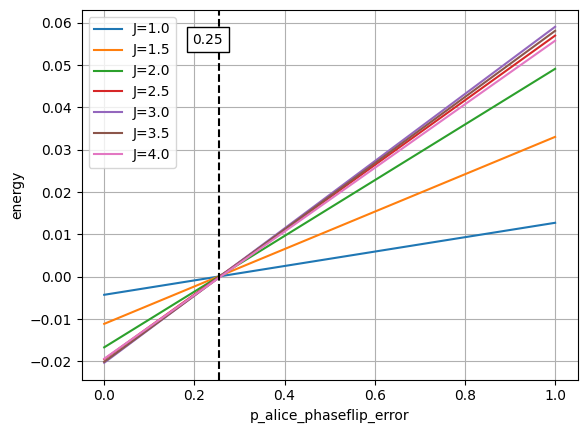
\includegraphics[width=\textwidth]{Appendix/plots/errors/numerical/NearestNeighbors/N2/Y_N2_energy_vs_p_alice_phaseflip_error.png}
        \caption{Energy, $N=2$}
    \end{subfigure}
    \hfill
    \begin{subfigure}[b]{0.29\textwidth}
        \centering
        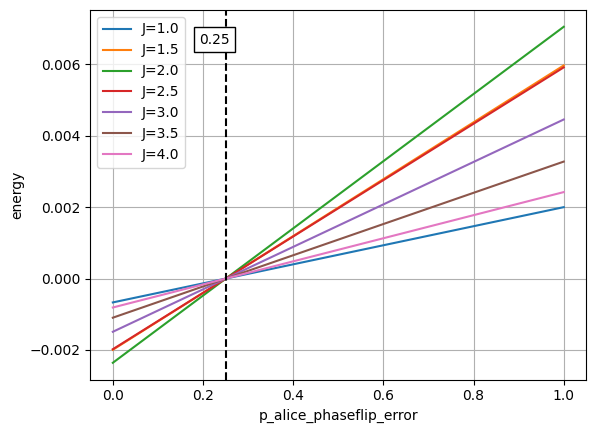
\includegraphics[width=\textwidth]{Appendix/plots/errors/numerical/NearestNeighbors/N3/Y_N3_energy_vs_p_alice_phaseflip_error.png}
        \caption{Energy, $N=3$}
    \end{subfigure}
    \hfill
    \begin{subfigure}[b]{0.29\textwidth}
        \centering
        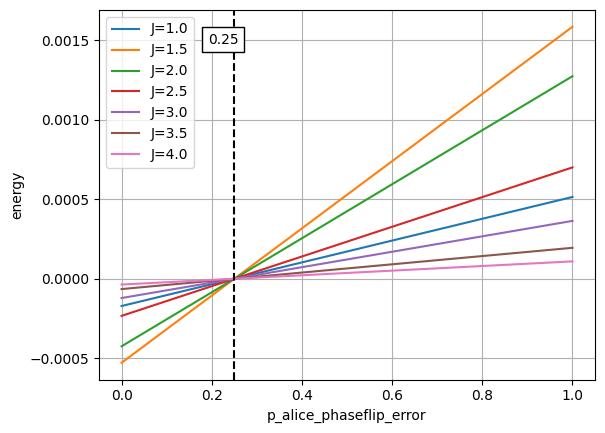
\includegraphics[width=\textwidth]{Appendix/plots/errors/numerical/NearestNeighbors/N4/Y_N4_energy_vs_p_alice_phaseflip_error.png}
        \caption{Energy, $N=4$}
    \end{subfigure}

    \vspace{0.5em}

    \begin{subfigure}[b]{0.29\textwidth}
        \centering
        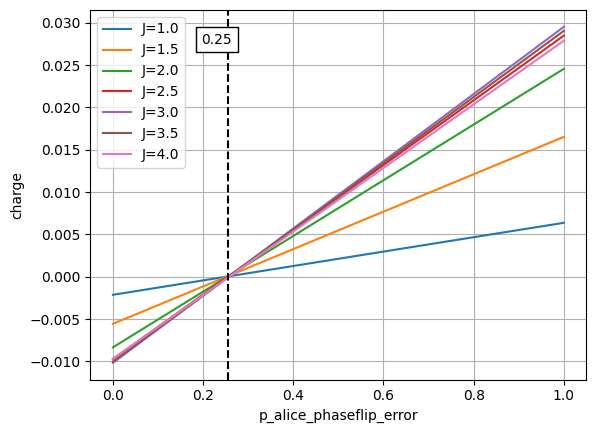
\includegraphics[width=\textwidth]{Appendix/plots/errors/numerical/NearestNeighbors/N2/Y_N2_charge_vs_p_alice_phaseflip_error.png}
        \caption{Charge, $N=2$}
    \end{subfigure}
    \hfill
    \begin{subfigure}[b]{0.29\textwidth}
        \centering
        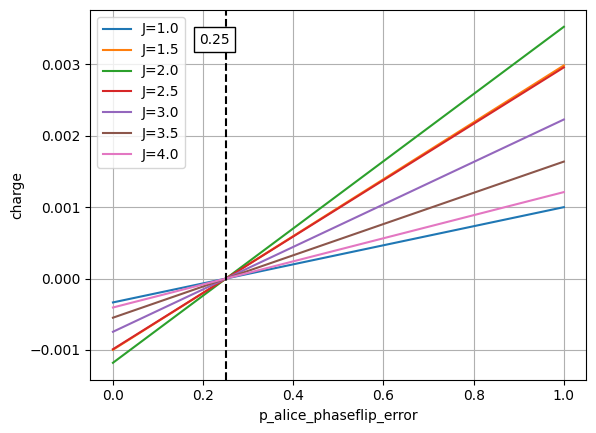
\includegraphics[width=\textwidth]{Appendix/plots/errors/numerical/NearestNeighbors/N3/Y_N3_charge_vs_p_alice_phaseflip_error.png}
        \caption{Charge, $N=3$}
    \end{subfigure}
    \hfill
    \begin{subfigure}[b]{0.29\textwidth}
        \centering
        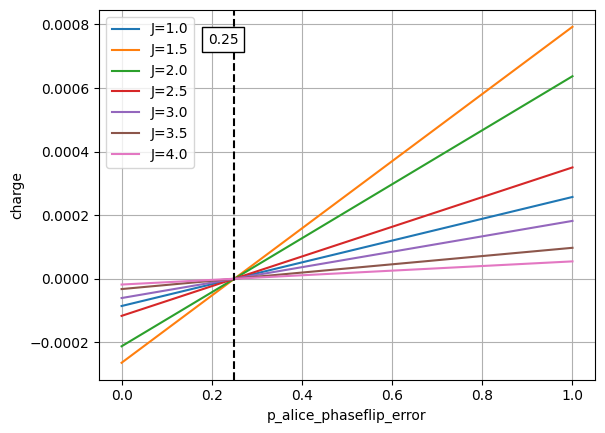
\includegraphics[width=\textwidth]{Appendix/plots/errors/numerical/NearestNeighbors/N4/Y_N4_charge_vs_p_alice_phaseflip_error.png}
        \caption{Charge, $N=4$}
    \end{subfigure}
    
    \caption{Numerical simulation results for teleported expectation value vs. the probability $p$ of phaseflip at Alice's site for Nearest Neighbors Hamiltonian \(H^{(2)}\) with Alice base \(\sigma_A = Y_0\).}
    \label{fig:nn_Y_num_alice_phaseflip_error_appendix}
\end{figure*}

\begin{figure*}[tb!]
    \centering
    \begin{subfigure}[b]{0.24\textwidth}
        \centering
        
\includegraphics[width=\textwidth]{Appendix/plots/errors/qiskit/NearestNeighbors/N2/X_N2_energy_vs_p_alice_phaseflip_error.png}
        \caption{Energy, $N=2$, $\sigma_A = X_0$}
    \end{subfigure}
    \hfill
    \begin{subfigure}[b]{0.24\textwidth}
        \centering
        
\includegraphics[width=\textwidth]{Appendix/plots/errors/qiskit/NearestNeighbors/N3/X_N3_energy_vs_p_alice_phaseflip_error.png}
        \caption{Energy, $N=3$, $\sigma_A = X_0$}
    \end{subfigure}
    \hfill
    \begin{subfigure}[b]{0.24\textwidth}
        \centering
        
\includegraphics[width=\textwidth]{plots/errors/qiskit/N2_charge_vs_p_alice_phaseflip_error.png}
        \caption{Charge, $N=2$, $\sigma_A = X_0$}
    \end{subfigure}
    \hfill
    \begin{subfigure}[b]{0.24\textwidth}
        \centering
        
\includegraphics[width=\textwidth]{Appendix/plots/errors/qiskit/NearestNeighbors/N3/X_N3_charge_vs_p_alice_phaseflip_error.png}
        \caption{Charge, $N=3$, $\sigma_A = X_0$}
    \end{subfigure}

    \vspace{0.5em}

    \begin{subfigure}[b]{0.24\textwidth}
        \centering
        
\includegraphics[width=\textwidth]{Appendix/plots/errors/qiskit/NearestNeighbors/N2/Y_N2_energy_vs_p_alice_phaseflip_error.png}
        \caption{Energy, $N=2$, $\sigma_A = Y_0$}
    \end{subfigure}
    \hfill
    \begin{subfigure}[b]{0.24\textwidth}
        \centering
        
\includegraphics[width=\textwidth]{Appendix/plots/errors/qiskit/NearestNeighbors/N3/Y_N3_energy_vs_p_alice_phaseflip_error.png}
        \caption{Energy, $N=3$, $\sigma_A = Y_0$}
    \end{subfigure}
    \hfill
    \begin{subfigure}[b]{0.24\textwidth}
        \centering
        
\includegraphics[width=\textwidth]{Appendix/plots/errors/qiskit/NearestNeighbors/N2/Y_N2_charge_vs_p_alice_phaseflip_error.png}
        \caption{Charge, $N=2$, $\sigma_A = Y_0$}
    \end{subfigure}
    \hfill
    \begin{subfigure}[b]{0.24\textwidth}
        \centering
        
\includegraphics[width=\textwidth]{Appendix/plots/errors/qiskit/NearestNeighbors/N3/Y_N3_charge_vs_p_alice_phaseflip_error.png}
        \caption{Charge, $N=3$, $\sigma_A = Y_0$}
    \end{subfigure}
    
    \caption{Qiskit simulation results for teleported expectation value vs. the probability $p$ of phaseflip at Alice's site for Nearest Neighbors Hamiltonian \(H^{(2)}\) for both Alice bases.}
    \label{fig:nn_qiskit_alice_phaseflip_error_appendix}
\end{figure*}


A phase-flip error on Alice's qubit, modeled by the channel $\rho \rightarrow (1-p)\rho + pZ_{0}\rho Z_{0}$, represents a significant threat to the protocol's integrity. The impact of this error is fundamentally different from a bit-flip, as it directly interferes with the measurement process itself.

The physical mechanism behind this vulnerability is the decoherence of Alice's measurement basis \cite{QKDbyQET, Lydersen2010, Zhao2008}. Alice performs her measurement in a basis (e.g., $\sigma_A = X_0$ or $Y_0$) that anticommutes with the phase-flip operator $Z_0$. This error randomizes the phase relationship between the eigenstates of Alice's measurement, degrading her ability to accurately project the shared state. This directly suppresses the expectation value of the correlator that forms the "engine" of the teleportation, $\eta = i\langle[O_B, \sigma_B]\sigma_A\rangle$. As $\eta$ is responsible for generating the negative signal at Bob's side, its attenuation causes the teleported expectation value to degrade and shift towards positive values.

The simulation results presented in Figures \ref{fig:alice_num_alice_phaseflip_error_appendix} through \ref{fig:nn_qiskit_alice_phaseflip_error_appendix} confirm this behavior. 
\begin{itemize}
    \item Across all models and parameters, a phase-flip error on Alice's qubit leads to a roughly linear degradation of the teleported signal, for both energy and charge. Unlike the more benign bit-flip error, this degradation is severe enough to cause a sign-flip at a relatively low error probability, representing a failure of the QKD protocol.
    
    \item The critical threshold where the signal crosses zero is consistently found in the range of $p \approx 0.25-0.33$, as seen in the numerical plots. This indicates that both energy and charge teleportation protocols are similarly vulnerable to this type of noise.
    
    \item The Qiskit simulations in Figures \ref{fig:alice_qiskit_alice_phaseflip_error_appendix} and \ref{fig:nn_qiskit_alice_phaseflip_error_appendix} validate the trends observed in the ideal numerical calculations. They reproduce the signal attenuation and eventual sign-flip, demonstrating that this vulnerability persists in circuit-level implementations, albeit with additional statistical noise.
\end{itemize}
In summary, a phase-flip error on Alice's qubit is a detrimental noise source that attacks the core mechanism of the teleportation protocol by decohering the measurement basis. Its impact is severe for both energy and charge observables, establishing a critical error threshold beyond which secure key distribution is not possible.

\subsection{Bob site Phase-Flip Error}

\begin{figure*}[tb!]
    \centering
    \subfloat[Energy, \( N = 1 \)]{
        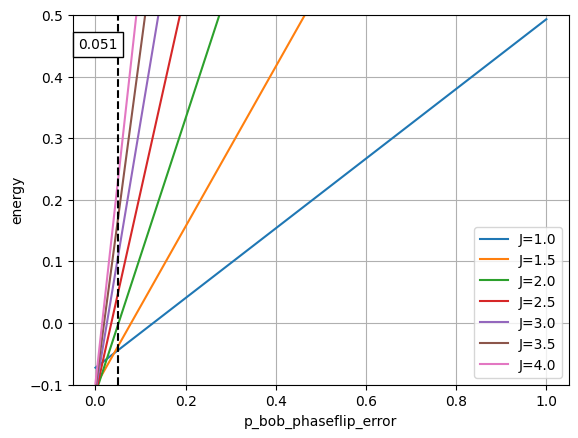
\includegraphics[width=0.225\textwidth]{Appendix/plots/errors/numerical/Alice/N1/N1_energy_vs_p_bob_phaseflip_error.png}
    }
    \hfill
    \subfloat[Energy, \( N = 2 \)]{
        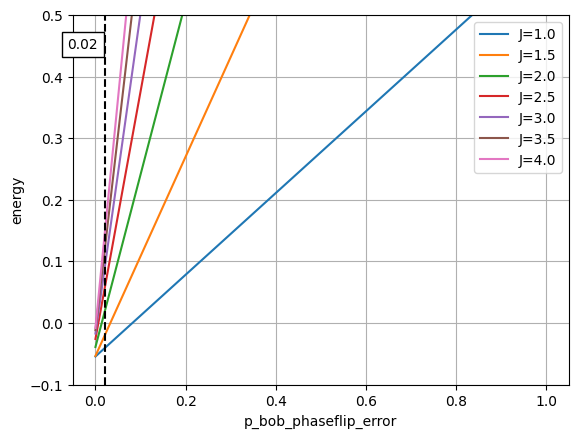
\includegraphics[width=0.225\textwidth]{Appendix/plots/errors/numerical/Alice/N2/N2_energy_vs_p_bob_phaseflip_error.png}
    }
    \hfill
    \subfloat[Energy, \( N = 3 \)]{
        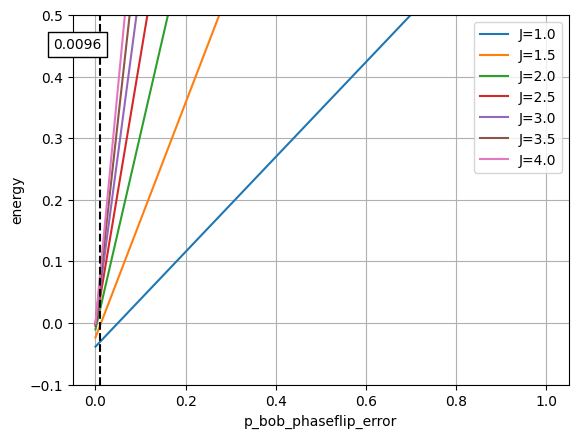
\includegraphics[width=0.225\textwidth]{Appendix/plots/errors/numerical/Alice/N3/N3_energy_vs_p_bob_phaseflip_error.png}
    }
    \hfill
    \subfloat[Energy, \( N = 4 \)]{
        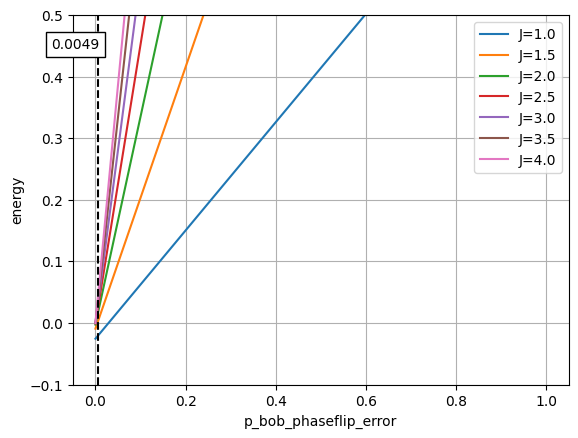
\includegraphics[width=0.225\textwidth]{Appendix/plots/errors/numerical/Alice/N4/N4_energy_vs_p_bob_phaseflip_error.png}
    }

    \vspace{0.5em}

    \subfloat[Charge, \( N = 1 \)]{
        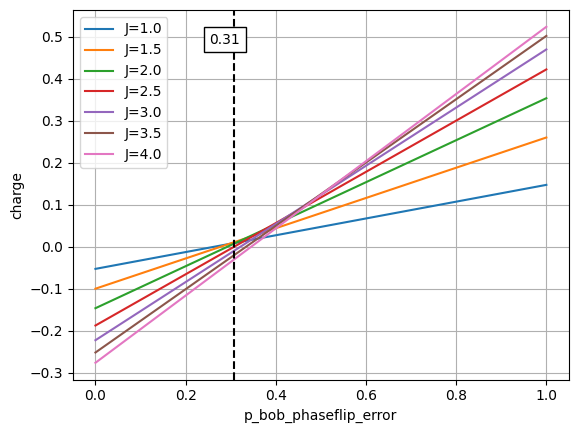
\includegraphics[width=0.225\textwidth]{Appendix/plots/errors/numerical/Alice/N1/N1_charge_vs_p_bob_phaseflip_error.png}
    }
    \hfill
    \subfloat[Charge, \( N = 2 \)]{
        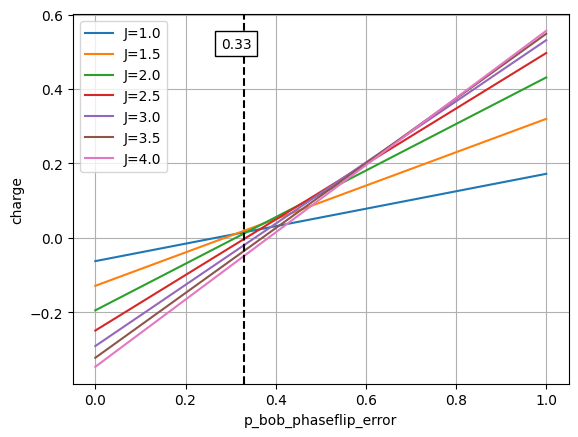
\includegraphics[width=0.225\textwidth]{Appendix/plots/errors/numerical/Alice/N2/N2_charge_vs_p_bob_phaseflip_error.png}
    }
    \hfill
    \subfloat[Charge, \( N = 3 \)]{
        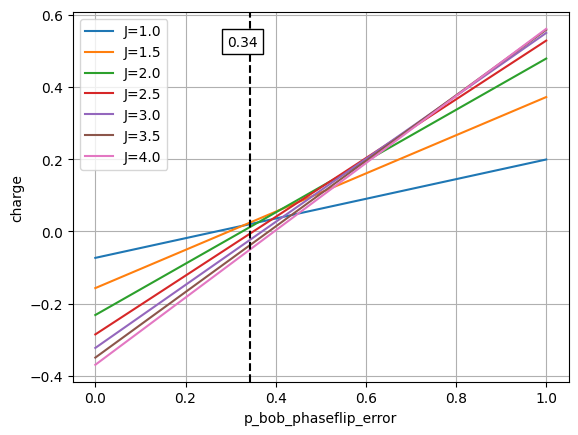
\includegraphics[width=0.225\textwidth]{Appendix/plots/errors/numerical/Alice/N3/N3_charge_vs_p_bob_phaseflip_error.png}
    }
    \hfill
    \subfloat[Charge, \( N = 4 \)]{
        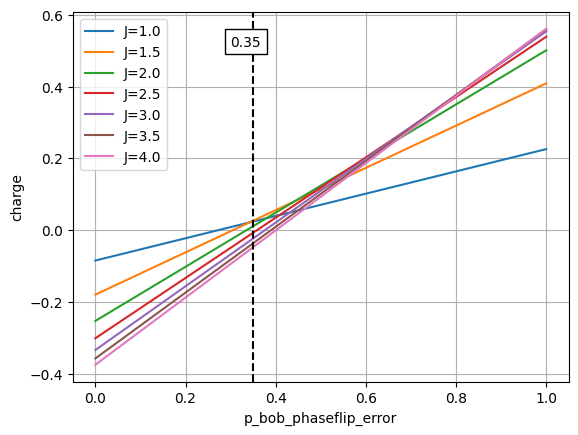
\includegraphics[width=0.225\textwidth]{Appendix/plots/errors/numerical/Alice/N4/N4_charge_vs_p_bob_phaseflip_error.png}
    }
    
    \caption{Numerical simulation results for teleported expectation value vs. the probability $p$ of phaseflip at Bob's site for Star-Interaction Hamiltonian \(H^{(1)}\).}
    \label{fig:alice_num_bob_phaseflip_error_appendix}
\end{figure*}

\begin{figure*}[tb!]
    \centering
    \subfloat[Energy, \( N = 1 \)]{
        
\includegraphics[width=0.3\textwidth]{Appendix/plots/errors/qiskit/Alice/N1/N1_energy_vs_p_bob_phaseflip_error.png}
    }
    \hfill
    \subfloat[Energy, \( N = 2 \)]{
        
\includegraphics[width=0.3\textwidth]{Appendix/plots/errors/qiskit/Alice/N2/N2_energy_vs_p_bob_phaseflip_error.png}
    }
    \hfill
    \subfloat[Energy, \( N = 3 \)]{
        
\includegraphics[width=0.3\textwidth]{Appendix/plots/errors/qiskit/Alice/N3/N3_energy_vs_p_bob_phaseflip_error.png}
    }

    \vspace{0.5em}

    \subfloat[Charge, \( N = 1 \)]{
        
\includegraphics[width=0.3\textwidth]{Appendix/plots/errors/qiskit/Alice/N1/N1_charge_vs_p_bob_phaseflip_error.png}
    }
    \hfill
    \subfloat[Charge, \( N = 2 \)]{
        
\includegraphics[width=0.3\textwidth]{Appendix/plots/errors/qiskit/Alice/N2/N2_charge_vs_p_bob_phaseflip_error.png}
    }
    \hfill
    \subfloat[Charge, \( N = 3 \)]{
        
\includegraphics[width=0.3\textwidth]{Appendix/plots/errors/qiskit/Alice/N3/N3_charge_vs_p_bob_phaseflip_error.png}
    }
    
    \caption{Qiskit simulation results for teleported expectation value vs. the probability $p$ of phaseflip at Bob's site for Star-Interaction Hamiltonian \(H^{(1)}\).}
    \label{fig:alice_qiskit_bob_phaseflip_error_appendix}
\end{figure*}

\begin{figure*}[tb!]
    \centering
    \subfloat[Energy, \( N = 2 \)]{
        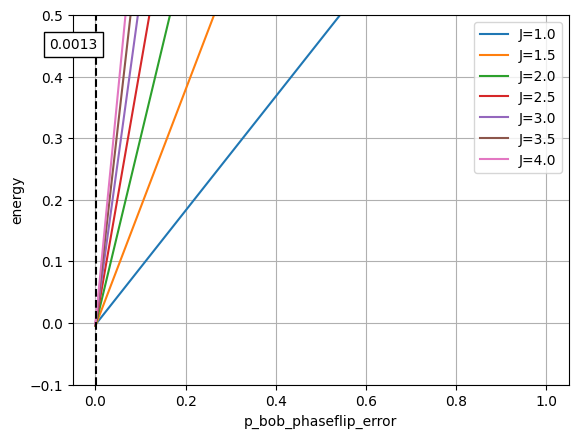
\includegraphics[width=0.3\textwidth]{Appendix/plots/errors/numerical/NearestNeighbors/N2/X_N2_energy_vs_p_bob_phaseflip_error.png}
    }
    \hfill
    \subfloat[Energy, \( N = 3 \)]{
        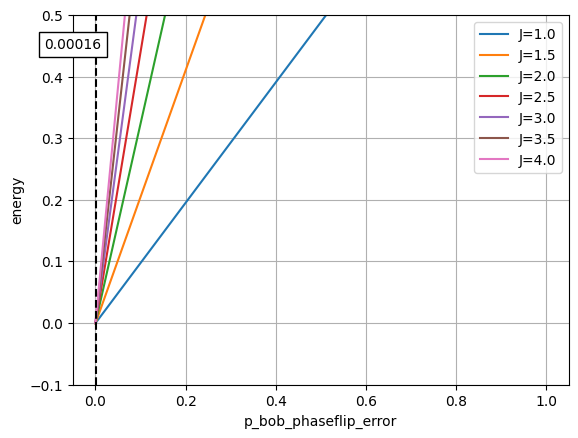
\includegraphics[width=0.3\textwidth]{Appendix/plots/errors/numerical/NearestNeighbors/N3/X_N3_energy_vs_p_bob_phaseflip_error.png}
    }
    \hfill
    \subfloat[Energy, \( N = 4 \)]{
        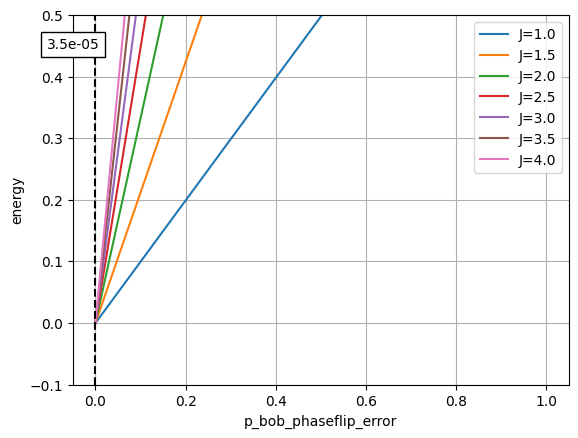
\includegraphics[width=0.3\textwidth]{Appendix/plots/errors/numerical/NearestNeighbors/N4/X_N4_energy_vs_p_bob_phaseflip_error.png}
    }

    \vspace{0.5em}

    \subfloat[Charge, \( N = 2 \)]{
        
\includegraphics[width=0.3\textwidth]{plots/errors/numerical/N2_charge_vs_p_bob_phaseflip_error.png}
    }
    \hfill
    \subfloat[Charge, \( N = 3 \)]{
        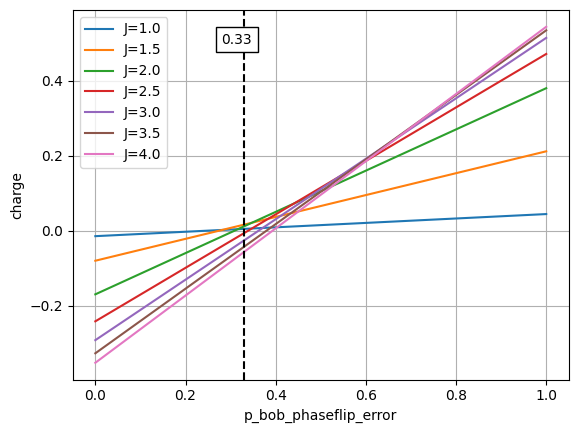
\includegraphics[width=0.3\textwidth]{Appendix/plots/errors/numerical/NearestNeighbors/N3/X_N3_charge_vs_p_bob_phaseflip_error.png}
    }
    \hfill
    \subfloat[Charge, \( N = 4 \)]{
        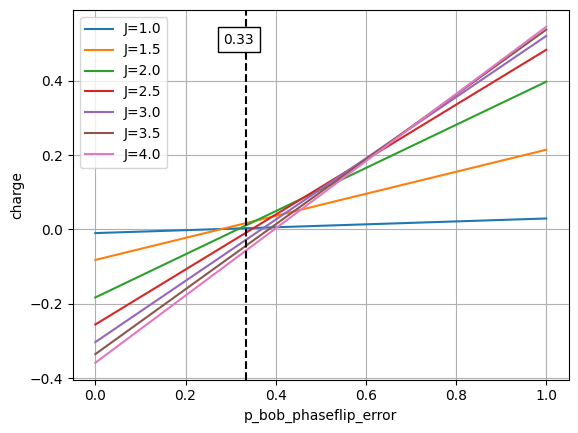
\includegraphics[width=0.3\textwidth]{Appendix/plots/errors/numerical/NearestNeighbors/N4/X_N4_charge_vs_p_bob_phaseflip_error.png}
    }
    
    \caption{Numerical simulation results for teleported expectation value vs. the probability $p$ of phaseflip at Bob's site for Nearest Neighbors Hamiltonian \(H^{(2)}\) with Alice base \(\sigma_A = X_0\).}
    \label{fig:nn_X_num_bob_phaseflip_error_appendix}
\end{figure*}

\begin{figure*}[tb!]
    \centering
    \subfloat[Energy, \( N = 2 \)]{
        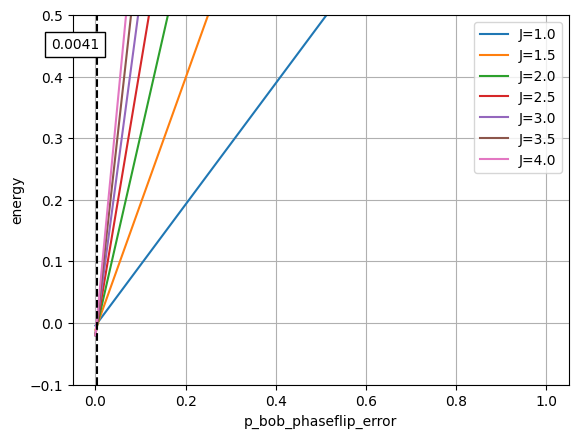
\includegraphics[width=0.3\textwidth]{Appendix/plots/errors/numerical/NearestNeighbors/N2/Y_N2_energy_vs_p_bob_phaseflip_error.png}
    }
    \hfill
    \subfloat[Energy, \( N = 3 \)]{
        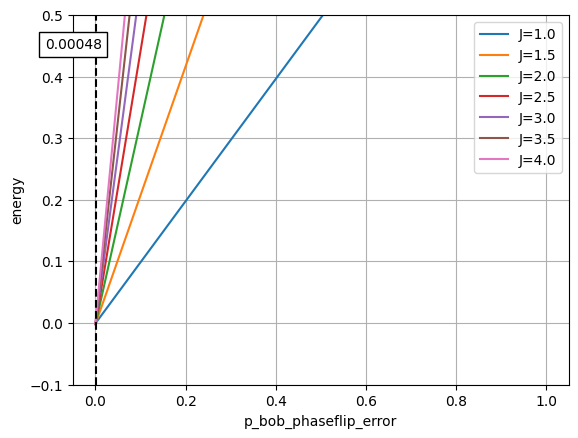
\includegraphics[width=0.3\textwidth]{Appendix/plots/errors/numerical/NearestNeighbors/N3/Y_N3_energy_vs_p_bob_phaseflip_error.png}
    }
    \hfill
    \subfloat[Energy, \( N = 4 \)]{
        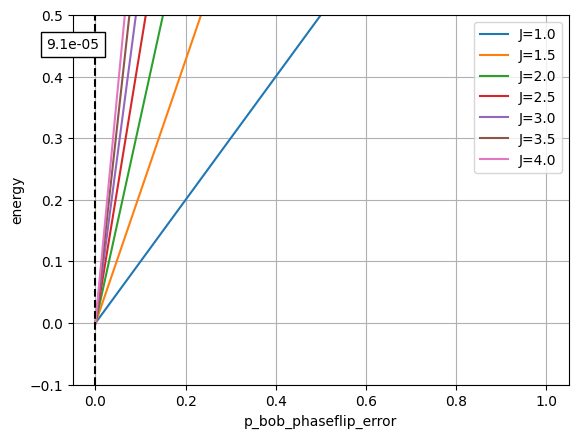
\includegraphics[width=0.3\textwidth]{Appendix/plots/errors/numerical/NearestNeighbors/N4/Y_N4_energy_vs_p_bob_phaseflip_error.png}
    }

    \vspace{0.5em}

    \subfloat[Charge, \( N = 2 \)]{
        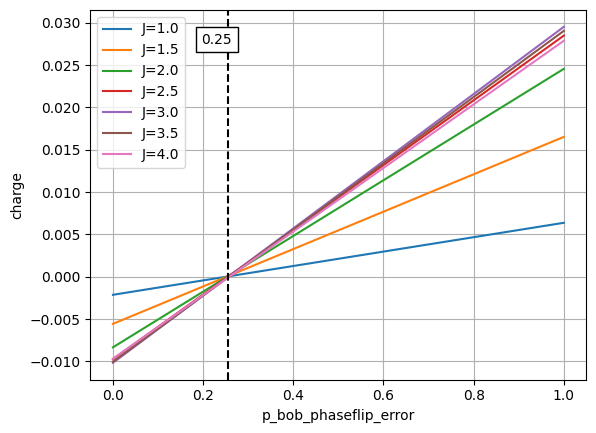
\includegraphics[width=0.3\textwidth]{Appendix/plots/errors/numerical/NearestNeighbors/N2/Y_N2_charge_vs_p_bob_phaseflip_error.png}
    }
    \hfill
    \subfloat[Charge, \( N = 3 \)]{
        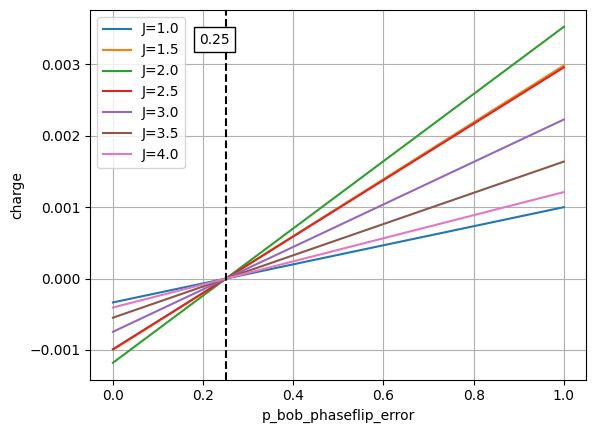
\includegraphics[width=0.3\textwidth]{Appendix/plots/errors/numerical/NearestNeighbors/N3/Y_N3_charge_vs_p_bob_phaseflip_error.png}
    }
    \hfill
    \subfloat[Charge, \( N = 4 \)]{
        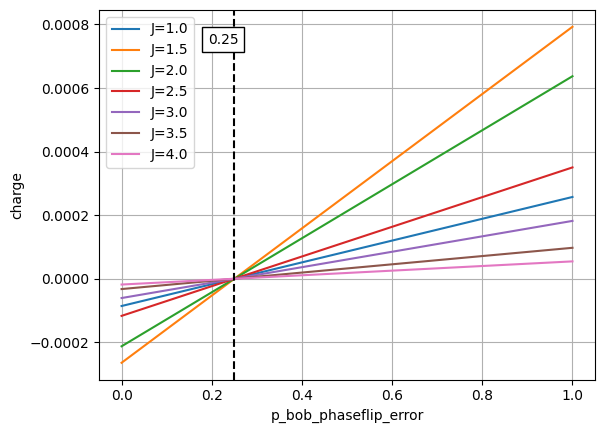
\includegraphics[width=0.3\textwidth]{Appendix/plots/errors/numerical/NearestNeighbors/N4/Y_N4_charge_vs_p_bob_phaseflip_error.png}
    }
    
    \caption{Numerical simulation results for teleported expectation value vs. the probability $p$ of phaseflip at Bob's site for Nearest Neighbors Hamiltonian \(H^{(2)}\) with Alice base \(\sigma_A = Y_0\).}
    \label{fig:nn_Y_num_bob_phaseflip_error_appendix}
\end{figure*}

\begin{figure*}[tb!]
    \centering
    \subfloat[Energy, \( N = 2 \), \( \sigma_A = X_0 \)]{
        
\includegraphics[width=0.225\textwidth]{Appendix/plots/errors/qiskit/NearestNeighbors/N2/X_N2_energy_vs_p_bob_phaseflip_error.png}
    }
    \hfill
    \subfloat[Energy, \( N = 3 \), \( \sigma_A = X_0 \)]{
        
\includegraphics[width=0.225\textwidth]{Appendix/plots/errors/qiskit/NearestNeighbors/N3/X_N3_energy_vs_p_bob_phaseflip_error.png}
    }
    \hfill
    \subfloat[Charge, \( N = 2 \), \( \sigma_A = X_0 \)]{
        
\includegraphics[width=0.225\textwidth]{plots/errors/qiskit/N2_charge_vs_p_bob_phaseflip_error.png}
    }
    \hfill
    \subfloat[Charge, \( N = 3 \), \( \sigma_A = X_0 \)]{
        
\includegraphics[width=0.225\textwidth]{Appendix/plots/errors/qiskit/NearestNeighbors/N3/X_N3_charge_vs_p_bob_phaseflip_error.png}
    }

    \vspace{0.5em}

    \subfloat[Energy, \( N = 2 \), \( \sigma_A = Y_0 \)]{
        
\includegraphics[width=0.225\textwidth]{Appendix/plots/errors/qiskit/NearestNeighbors/N2/Y_N2_energy_vs_p_bob_phaseflip_error.png}
    }
    \hfill
    \subfloat[Energy, \( N = 3 \), \( \sigma_A = Y_0 \)]{
        
\includegraphics[width=0.225\textwidth]{Appendix/plots/errors/qiskit/NearestNeighbors/N3/Y_N3_energy_vs_p_bob_phaseflip_error.png}
    }
    \hfill
    \subfloat[Charge, \( N = 2 \), \( \sigma_A = Y_0 \)]{
        
\includegraphics[width=0.225\textwidth]{Appendix/plots/errors/qiskit/NearestNeighbors/N2/Y_N2_charge_vs_p_bob_phaseflip_error.png}
    }
    \hfill
    \subfloat[Charge, \( N = 3 \), \( \sigma_A = Y_0 \)]{
        
\includegraphics[width=0.225\textwidth]{Appendix/plots/errors/qiskit/NearestNeighbors/N3/Y_N3_charge_vs_p_bob_phaseflip_error.png}
    }
    
    \caption{Qiskit simulation results for teleported expectation value vs. the probability $p$ of phaseflip at Bob's site for Nearest Neighbors Hamiltonian \(H^{(2)}\) for both Alice bases.}
    \label{fig:nn_qiskit_bob_phaseflip_error_appendix}
\end{figure*}


A phase-flip error occurring at Bob's site ($n=N$), modeled by the channel $\rho \rightarrow (1-p)\rho + pZ_{N}\rho Z_{N}$, is particularly detrimental to the protocol. Unlike an error on Alice's qubit which degrades the measurement, an error on Bob's qubit directly sabotages his corrective operation.

The physical mechanism for this vulnerability lies in how the phase-flip operator interacts with Bob's conditional rotation. Bob's unitary operation is typically a rotation around the Y or X axis (e.g., $U_B(\theta) = e^{-i\theta\sigma_B}$ where $\sigma_B \in \{X_N, Y_N\}$). A phase-flip error transforms this rotation via conjugation:
\begin{equation*}
Z_N R_Y(\theta) Z_N^\dagger = R_Y(-\theta)
\end{equation*}
This transformation inverts the sign of Bob's rotation angle. The effect is physically equivalent to Bob receiving the wrong classical bit from Alice and applying the incorrect unitary based on that misinformation \cite{QKDbyQET}. This causes a direct and rapid mixing of the intended negative signal with the unwanted positive signal, leading to an accelerated decay towards failure.

This behavior is clearly demonstrated in the simulation results presented in Figures \ref{fig:alice_num_bob_phaseflip_error_appendix} through \ref{fig:nn_qiskit_bob_phaseflip_error_appendix}.
\begin{itemize}
    \item All plots show a strong, nearly linear degradation of the teleported signal as a function of the error probability $p$. This rapid decay is characteristic of an error that directly inverts the protocol's intended outcome.
    
    \item This error leads to a sharp sign-crossing, with a critical failure threshold consistently observed around $p \approx 0.32-0.33$. This low tolerance highlights the protocol's sensitivity to phase noise on the receiving qubit.
    
    \item Both energy and charge protocols are similarly vulnerable to this error, as it attacks the final step of the protocol (Bob's conditional rotation) which is fundamental to both. The Qiskit simulations (Figures \ref{fig:alice_qiskit_bob_phaseflip_error_appendix} and \ref{fig:nn_qiskit_bob_phaseflip_error_appendix}) validate this severe impact, confirming that this vulnerability is a primary concern for practical hardware implementations.
\end{itemize}
In conclusion, a phase-flip error on Bob's qubit is one of the most damaging forms of local noise for this QKD protocol, as it effectively mimics a classical communication error and causes a rapid failure of the key generation process.

% \textbf{Depolarization Error:} A depolarizing channel causes the signal to decay linearly with $(1-p)$ but does not flip its sign. As shown analytically in \cite{QKDbyQET} and confirmed in our simulations in Figure \ref{fig:depolarizing_error_appendix}, this error reduces the magnitude of the teleported signal but does not alter its sign. Therefore, the QET-based QKD protocol is fundamentally robust against depolarization, contingent on the signal remaining detectable above the hardware's noise floor.

% \begin{figure}[ht!]
%     \centering
%     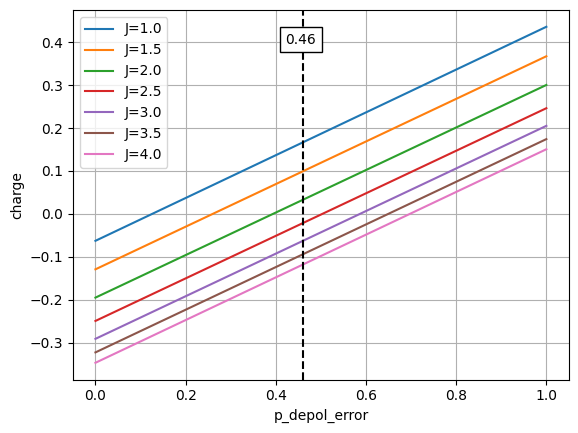
\includegraphics[width=0.6\textwidth]{Appendix/plots/errors/numerical/Alice/N2/N2_charge_vs_p_depol_error.png}
%     \caption{Effect of a depolarizing error on the resource state for the $H^{(1)}$ model with $N=2$. The teleported charge signal decays smoothly to zero as $p \to 1$ without crossing into positive values.}
%     \label{fig:depolarizing_error_appendix}
% \end{figure}